%% This is an example first chapter.  You should put chapter/appendix that you
%% write into a separate file, and add a line \include{yourfilename} to
%% main.tex, where `yourfilename.tex' is the name of the chapter/appendix file.
%% You can process specific files by typing their names in at the 
%% \files=
%% prompt when you run the file main.tex through LaTeX.

\singlespacing{

\chapter{Evaluation}\label{chap:evaluation}

Comparison with existing FEA methods revealed a similarity between the cell-cell interaction model I developed in Chapter \ref{chap:functionSim} and a shear-dominated 12DOF Timoshenko Beam Element (Section \ref{sec:Timoshenko}).  My model extends the shear-dominated Timoshenko model with non-linear handling of large angular deformations, rather than using small angle approximations.  I argue that this is an appropriate model given the aspect ratio of the parts I am modeling (Figure \ref{fig:StubbyBeam}) and the expected large angular deformations (Figure \ref{fig:deformationangle}).

\section{Comparison with FEA Techniques}\label{sec:Timoshenko}

\begin{figure}
  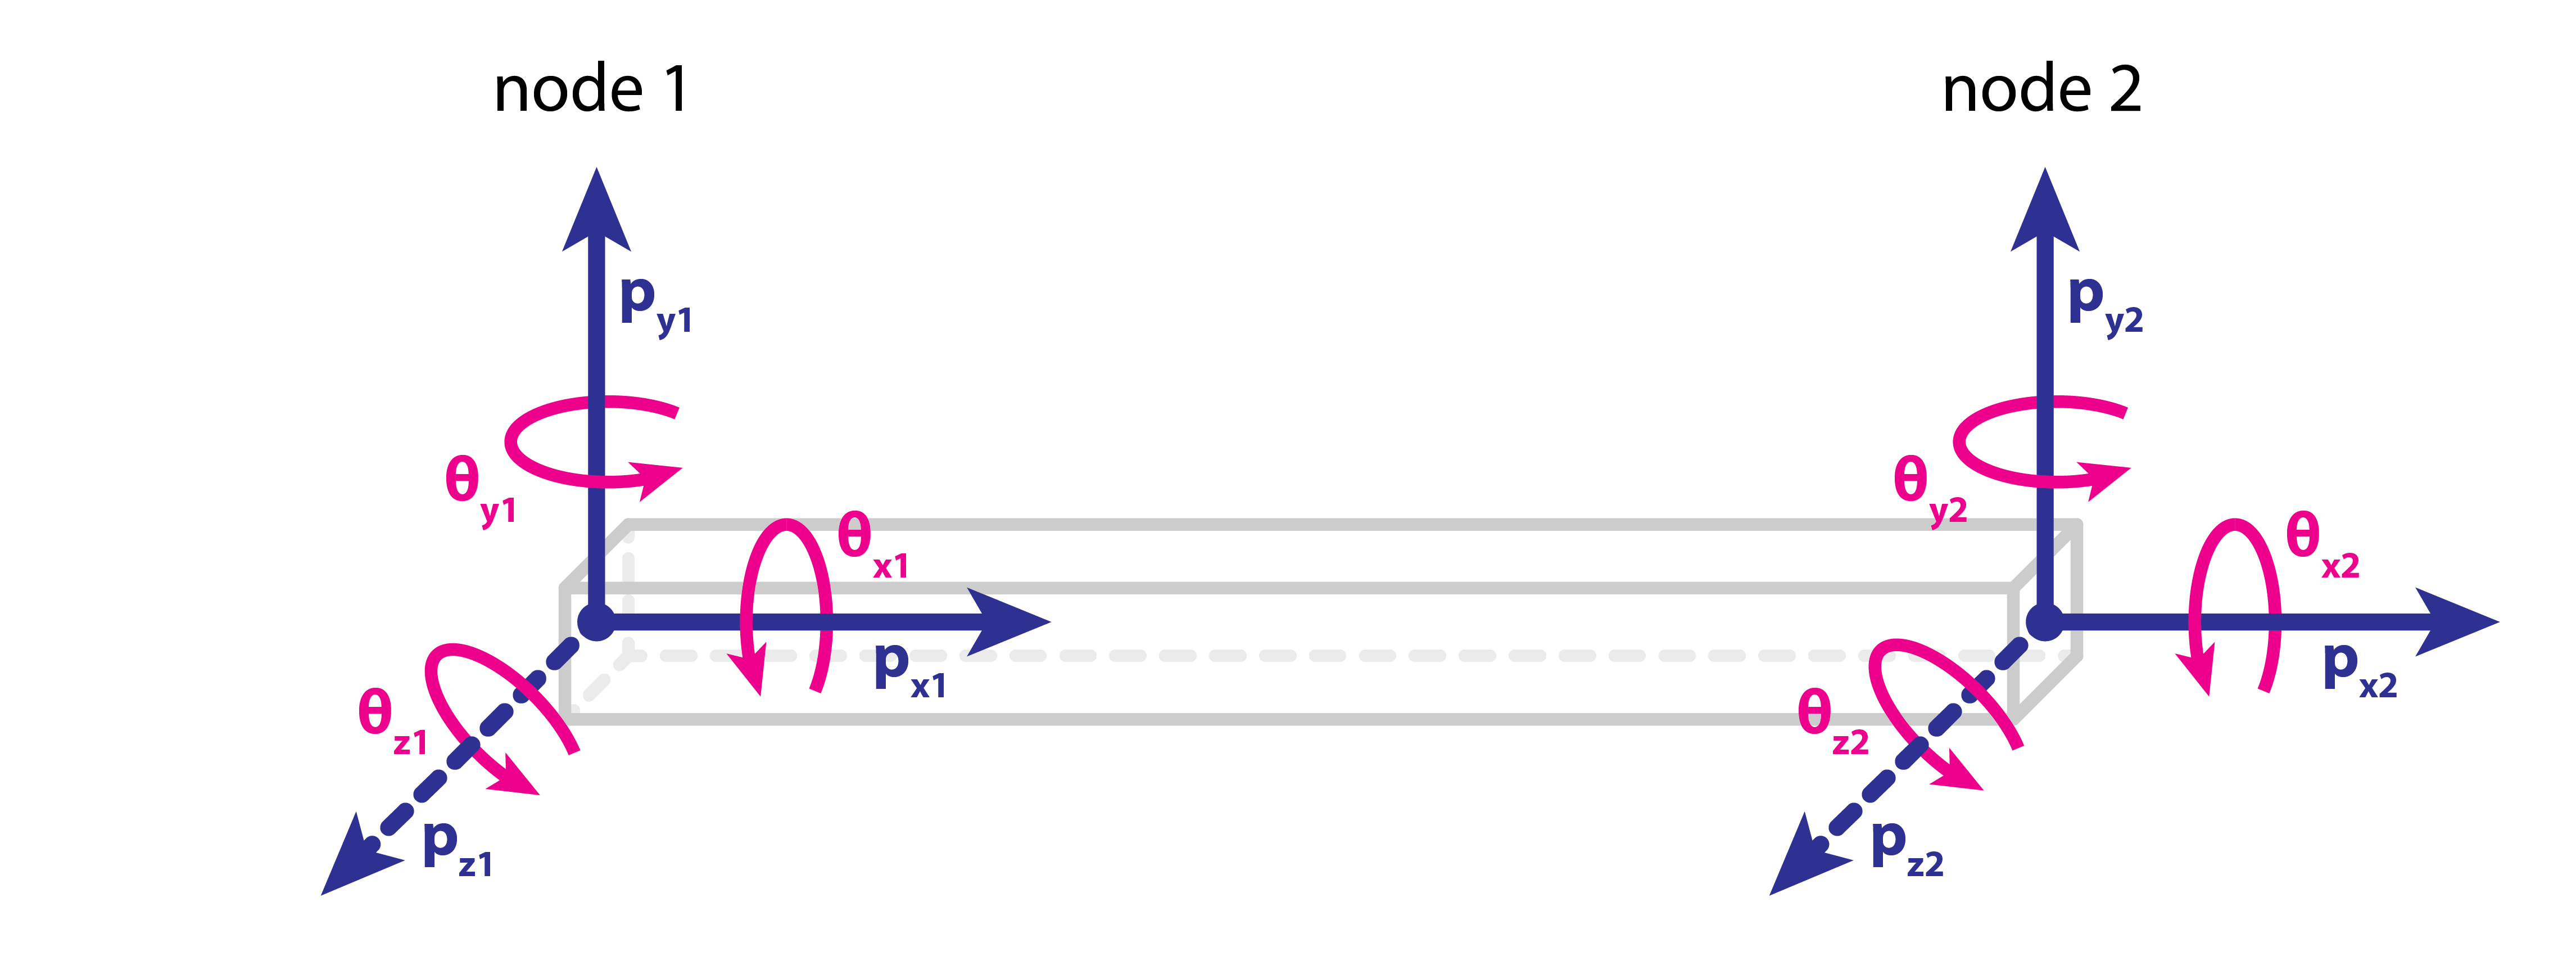
\includegraphics[width=\linewidth]{BeamSetup.png}
  \caption{Setup of 12DOF beam model connecting two nodes (nodes 1 and 2).  Translational displacement indicated by $p_x$, $p_y$, $p_z$ and angular displacement indicated by $\theta_x$, $\theta_y$, $\theta_z$.}
  \label{fig:BeamSetup}
\end{figure}

We can perform an analysis of the interactions between two cells using standard techniques from FEA to see how they compare with what we've derived in the previous sections.  Within FEA, many types of models are used to describe the behavior of linear elastic solids with varying degrees of accuracy and computational complexity.  One model that computes translational and rotational degrees of freedom between two nodes is the 12DOF Timoshenko beam.  Using this model, we can construct a beam element between two nodes that represents the material joining two adjacent cells.  The model determines the translational and rotational displacements of both nodes in 3D (Figure \ref{fig:BeamSetup}).  The Timoshenko beam element takes into account axial deformation, bending deformation with shear effects, and torsional deformation.\\  

\textit{Shape functions} are polynomials in 1D, 2D, or 3D that describe how the behavior of the nodes should be interpolated in the regions between the nodes (e.g. the inner volume of the tetrahedron in Figure \ref{fig:TetraElement}).  Hermitian cubic shape functions are typically used for beam models; they are third order polynomials that provide continuity between discretized solutions along nodes in a beam.  A graphical description of shape functions is shown in Wolfram \cite{Wolfram2016}.  The shape functions expressed in terms of a dimensionless coordinate $\xi$ are:
\begin{align*} 
N_{x1} &= \textstyle\frac{1}{4}(1-\xi)^2(2+\xi)\\
N_{x2} &= \textstyle\frac{1}{4}(1+\xi)^2(2-\xi)\\
N_{\theta1} &= \textstyle\frac{1}{8}l(1-\xi)^2(1+\xi)\\
N_{\theta2} &= \textstyle\frac{1}{8}l(1+\xi)^2(1-\xi)
\end{align*}

where $-1 \leq \xi \leq 1$ and $\xi = -1$ at node 1 and $\xi = 1$ at node 2\\

Using these shape functions we can calculate the \textit{stiffness matrix} ($K$) of the 12DOF Timoshenko beam oriented along the x-axis:\\

\[ K =  \scriptsize {\left[ \begin{smallmatrix}
\tfrac{EA}{l} & 0 & 0 & 0 & 0 & 0 & \tfrac{-EA}{l} & 0 & 0 & 0 & 0 & 0\\
 & \tfrac{12EI_z}{l^3(1+\phi_y)} & 0 & 0 & 0 & \tfrac{6EI_z}{l^2(1+\phi_y)} & 0 & \tfrac{-12EI_z}{l^3(1+\phi_y)} & 0 & 0 & 0 & \tfrac{6EI_z}{l^2(1+\phi_y)}\\
 &  & \tfrac{12EI_y}{l^3(1+\phi_z)} & 0 & \tfrac{-6EI_y}{l^2(1+\phi_z)} & 0 & 0 & 0 & \tfrac{-12EI_y}{l^3(1+\phi_z)} & 0 & \tfrac{-6EI_y}{l^2(1+\phi_z)} & 0\\
 &  &  &  \tfrac{GJ}{l} &  0 &  0 &  0 &  0 &  0 & \tfrac{-GJ}{l} & 0 & 0\\
 &  &  &  & \tfrac{(4+\phi_z)EI_y}{l(1+\phi_z)} & 0 & 0 & 0 & \tfrac{6EI_y}{l^2(1+\phi_z)} & 0 & \tfrac{(2-\phi_z)EI_y}{l(1+\phi_z)} & 0\\
 &  &  &  &  & \tfrac{(4+\phi_y)EI_z}{l(1+\phi_y)} & 0 & \tfrac{-6EI_z}{l^2(1+\phi_y)} & 0 & 0 & 0 & \tfrac{(2-\phi_y)EI_z}{l(1+\phi_y)}\\
 &  &  &  &  &  & \tfrac{EA}{l}  & 0 & 0 & 0 & 0 & 0\\
 &  &  &  &  &  &  & \tfrac{12EI_z}{l^3(1+\phi_y)} & 0 & 0 & 0 & \tfrac{-6EI_z}{l^2(1+\phi_y)}\\
 &  &  &  &  &  &  &  & \tfrac{12EI_y}{l^3(1+\phi_z)} & 0 & \tfrac{6EI_y}{l^2(1+\phi_z)}\ & 0\\
 &  & symmetric &  &  &  &  &  &  & \tfrac{GJ}{l} & 0 & 0\\
 &  &  &  &  &  &  &  &  &  & \tfrac{(4+\phi_z)EI_y}{l(1+\phi_z)} & 0\\
  &  &  &  &  &  &  &  &  &  &  & \tfrac{(4+\phi_y)EI_z}{l(1+\phi_y)}\\
 \end{smallmatrix} \right] }\]
 
 where
\[ \phi_y = \dfrac{12EI_z}{GA_{sy}l^2} \qquad  \textrm{and} \qquad \phi_z = \dfrac{12EI_y}{GA_{sz}l^2} \]


The stiffness matrix gives us a way to convert between translational/rotational nodal displacements and forces, according to the following equation:

 \begin{equation} \label{eq:forcestiffnessdisp} \vec{F} = -K\vec{u} \end{equation}
where:
\[ \vec{F} =  \left[ \begin{array}{ccc}
F_{x1}\\
F_{y1}\\
F_{z1}\\
T_{x1}\\
T_{y1}\\
T_{z1}\\
F_{x2}\\
F_{y2}\\
F_{z2}\\
T_{x2}\\
T_{y2}\\
T_{z2}
 \end{array} \right]  \qquad \qquad  
 \vec{u} =  \left[ \begin{array}{ccc}
p_{x1}\\
p_{y1}\\
p_{z1}\\
\theta_{x1}\\
\theta_{y1}\\
\theta_{z1}\\
p_{x2}\\
p_{y2}\\
p_{z2}\\
\theta_{x2}\\
\theta_{y2}\\
\theta_{z2}
 \end{array} \right]
 \]\\
 
where $F_1$, $F_2$ are translational forces acting on nodes 1 and 2, $T$ are torques, $p$ are translational displacements, and $\theta$ are rotational displacements.  The negative sign was put in front of the stiffness matrix in Equation \ref{eq:forcestiffnessdisp} to keep the same convention of restoring forces used in Chapter \ref{chap:functionSim}.\\

Multiplying through Equation \ref{eq:forcestiffnessdisp} gives us 12 equations:

\begin{subequations}
\begin{align} 
\label{eq:fx1}
F_{x1} &=  -\dfrac{EA}{l}p_{x1} + \dfrac{EA}{l}p_{x2} \\[10pt]
\label{eq:fy1}
F_{y1} &=  -\dfrac{12EI_z}{l^3(1+\phi_y)}p_{y1} - \dfrac{6EI_z}{l^2(1+\phi_y)}\theta_{z1} + \dfrac{12EI_z}{l^3(1+\phi_y)}p_{y2} - \dfrac{6EI_z}{l^2(1+\phi_y)}\theta_{z2}\\[10pt]
\label{eq:fz1}
F_{z1} &=  -\dfrac{12EI_y}{l^3(1+\phi_z)}p_{z1} - \dfrac{6EI_y}{l^2(1+\phi_z)}\theta_{y1} + \dfrac{12EI_y}{l^3(1+\phi_z)}p_{z2} - \dfrac{6EI_y}{l^2(1+\phi_z)}\theta_{y2}\\[10pt]
\label{eq:tx1}
T_{x1} &=  -\dfrac{GJ}{l}\theta_{x1} + \dfrac{GJ}{l}\theta_{x2} \\[10pt]
\label{eq:ty1}
T_{y1} &= \dfrac{6EI_y}{l^2(1+\phi_z)}p_{z1} - \dfrac{(4+\phi_z)EI_y}{l(1+\phi_z)}\theta_{y1}  - \dfrac{6EI_y}{l^2(1+\phi_z)}p_{z2} - \dfrac{(2-\phi_z)EI_y}{l(1+\phi_z)}\theta_{y2} \\[10pt]
\label{eq:tz1}
T_{z1} &=  -\dfrac{6EI_z}{l^2(1+\phi_y)}p_{y1} - \dfrac{(4+\phi_y)EI_z}{l(1+\phi_y)}\theta_{z1}  + \dfrac{6EI_z}{l^2(1+\phi_y)}p_{y2} - \dfrac{(2-\phi_y)EI_z}{l(1+\phi_y)}\theta_{z2} \\[10pt]
\label{eq:fx2}
F_{x2} &=  -F_{x1}\\[10pt]
\label{eq:fy2}
F_{y2} &=  -F_{y1}\\[10pt]
\label{eq:fz2}
F_{z2} &=  -F_{z1}\\[10pt]
\label{eq:tx2}
T_{x2} &=  -T_{x1}\\[10pt]
\label{eq:ty2}
T_{y2} &=  \dfrac{6EI_y}{l^2(1+\phi_z)}p_{z1} - \dfrac{(2-\phi_z)EI_y}{l(1+\phi_z)}\theta_{y1}  - \dfrac{6EI_y}{l^2(1+\phi_z)}p_{z2} - \dfrac{(4+\phi_z)EI_y}{l(1+\phi_z)}\theta_{y2} \\[10pt]
\label{eq:tz2}
T_{z2} &= -\dfrac{6EI_z}{l^2(1+\phi_y)}p_{y1} - \dfrac{(2-\phi_y)EI_z}{l(1+\phi_y)}\theta_{z1}  + \dfrac{6EI_z}{l^2(1+\phi_y)}p_{y2} - \dfrac{(4+\phi_y)EI_z}{l(1+\phi_y)}\theta_{z2}
\end{align}
\end{subequations}\\

Combining Equations \ref{eq:fx1} and \ref{eq:kaxial} gives us the x-axis spring component of Equation \ref{eq:translationalEqOpp}, assuming no relative rotation between the nodes:
\[F_{x1} =  k_{axial_x}(p_{x2} - p_{x1}) \]

Equations \ref{eq:fy1} and \ref{eq:fz1} have the same general form.  Rearranging Equation \ref{eq:fy1} gives:
\begin{equation}\label{eq:Fy1decomp}
 F_{y1} =  \dfrac{12EI_z}{l^3(1+\phi_y)} (p_{y2} -p_{y1}) - \dfrac{6EI_z}{l^2(1+\phi_y)}(\theta_{z1} + \theta_{z2}) 
 \end{equation}

The force $F_{y1}$ acting on node 1 is a combination of contributions from bending and shear stiffnesses.  Assuming shear dominance, we can reduce Equation \ref{eq:Fy1decomp} to:
\[ F_{y1} =  \dfrac{12EI_z}{l^3\phi_y} (p_{y2} -p_{y1}) - \dfrac{6EI_z}{l^2\phi_y}(\theta_{z1} + \theta_{z2}) 
\]
\[ F_{y1} =  \dfrac{GA_{sy}}{l} (p_{y2} -p_{y1}) - \dfrac{GA_{sy}}{2}(\theta_{z1} + \theta_{z2}) 
\]

Substituting Equation \ref{eq:kshear} gives:

\[ F_{y1} =  k_{shear_{xy}} (p_{y2} -p_{y1}) - k_{shear_{xy}}l\dfrac{(\theta_{z1} + \theta_{z2})}{2}
\]

\[ F_{y1} =  k_{shear_{xy}} (p_{y2} -p_{y1} - l\theta_{z_{avg}})
\]

Which is a	 small angle approximation of the y-axis spring component of Equation \ref{eq:translationalEqOpp}.\\

We'll account for the bending components of Equation \ref{eq:Fy1decomp} in Section \ref{sec:bendingdominance}.\\

As discussed in Equation \ref{eq:translationalEqOpp}, the translational forces acting on node 1 are equal and opposite those acting on node 2.  This is summed up by Equations \ref{eq:fx2}, \ref{eq:fy2}, and \ref{eq:fz2}.\\

Combining Equations \ref{eq:tz1} and \ref{eq:ktorsion} gives us a small angle approximation to the x-axis rotational spring component of Equation \ref{eq:T1verbose} (in this case the small angle approximation reduces the first term of Equation \ref{eq:T1verbose} to zero, assuming that torques applied to node1 by node 2 have no x component):
\[T_{x1} =  k_{torsion_x}(\theta_{x2} - \theta_{x1}) \]

Equations \ref{eq:ty1} and \ref{eq:tz1} have the same general form.  Rearranging Equation \ref{eq:ty1} gives:
\begin{equation}\label{eq:Ty1decomp}
T_{y1} = - \dfrac{6EI_y}{l^2(1+\phi_z)}(p_{z2}- p_{z1}) - \dfrac{EI_y}{l(1+\phi_z)}((4+\phi_z)\theta_{y1}  + (2-\phi_z)\theta_{y2})
\end{equation}

As with Equation \ref{eq:Fy1decomp}, this is a combination of shear and bending effects.  Assuming shearing dominance reduces \ref{eq:Ty1decomp} to:
\begin{equation}\label{eq:Ty1decomp2}
T_{y1} = - \dfrac{6EI_y}{l^2\phi_z}(p_{z2}- p_{z1}) - \dfrac{EI_y}{l}(\theta_{y1}  - \theta_{y2})
\end{equation}

\[T_{y1} = - \dfrac{GA_{sz}}{2}(p_{z2}- p_{z1}) + \dfrac{EI_y}{l}(\theta_{y2}  - \theta_{y1})\]

Substituting Equation \ref{eq:kshear} and \ref{eq:kbending} gives:
\[T_{y1} = \dfrac{-l}{2}k_{shear_{xz}}(p_{z2}- p_{z1}) + k_{bending_y}(\theta_{y2}  - \theta_{y1})\]

which is a small angle approximation of the y-axis spring component of \ref{eq:T1verbose} with:
\[ \vec{l}_{rot12} \approx \vec{l}_{nom12} = \left[ \begin{array}{ccc}
-l\\
0\\
0
 \end{array} \right]\]
 
Following this same procedure with Equation \ref{eq:tz1} gives a similar result, but with an extra negative sign:
\[T_{z1} = (-)\dfrac{-l}{2}k_{shear_{xy}}(p_{y2}- p_{y1}) + k_{bending_z}(\theta_{z2}  - \theta_{z1})\]
 
This negative is a byproduct of the crossproduct in Equation \ref{eq:T1verbose}, according to the following unit vector relationships:
\begin{equation}\label{eq:crossUnits}
\hat{x} \times \hat{y} = \hat{z}  \qquad \hat{x} \times \hat{z} = -\hat{y}  
\end{equation}

We'll account for the bending components of Equation \ref{eq:Ty1decomp} in Section \ref{sec:bendingdominance}.\\

Finally, Equation \ref{eq:ty2} and \ref{eq:tz2} have the same general form. Rearranging Equation \ref{eq:ty2} gives:
\begin{equation}\label{eq:Ty2Decomp}
T_{y2} =  -\dfrac{6EI_y}{l^2(1+\phi_z)}(p_{z2} - p_{z1}) - \dfrac{EI_y}{l(1+\phi_z)}((2-\phi_z)\theta_{y1}  + (4+\phi_z)\theta_{y2})
\end{equation}

In the case of shearing dominance, \ref{eq:Ty2Decomp} reduces to:
\[  T_{y2} =  -\dfrac{6EI_y}{l^2\phi_z}(p_{z2} - p_{z1}) - \dfrac{EI_y}{l}(\theta_{y2}  - \theta_{y1}) \]

\[  T_{y2} =  \dfrac{GA_{sz}}{2}(p_{z1} - p_{z2}) + \dfrac{EI_y}{l}(\theta_{y1}  - \theta_{y2}) \]

Substituting Equation \ref{eq:kshear} and \ref{eq:kbending} gives:
\[  T_{y2} =  \dfrac{l}{2}k_{shear_{xz}}(p_{z1} - p_{z2}) + k_{bending_y}(\theta_{y1}  - \theta_{y2}) \]

which is a small angle approximation of the y-axis spring component of \ref{eq:T2verbose} with:
\[ \vec{l}_{rot21} \approx \vec{l}_{nom21} = \left[ \begin{array}{ccc}
l\\
0\\
0
 \end{array} \right]\]

Following this same procedure with \ref{eq:tz2}, we get:
\[  T_{z2} =  (-)\dfrac{l}{2}k_{shear_{xy}}(p_{y1} - p_{y2}) + k_{bending_z}(\theta_{z1}  - \theta_{z2}) \]

where again, the extra negative sign is accounted for by the cross product in Equation \ref{eq:T2verbose} and the relationships \ref{eq:crossUnits}.\\

Again, we'll account for the bending components of Equation \ref{eq:Ty2Decomp} in Section \ref{sec:bendingdominance}.\\

Through this process, we have also shown that for shearing dominance, y and z components of torque (Equations \ref{eq:ty1}, \ref{eq:tz1}, \ref{eq:ty2}, \ref{eq:tz2}) of one node are equal and opposite to the other node (Equation \ref{eq:torqueEqOpp}).

\subsection{Missing Bending Contributions}\label{sec:bendingdominance}

\begin{figure}
  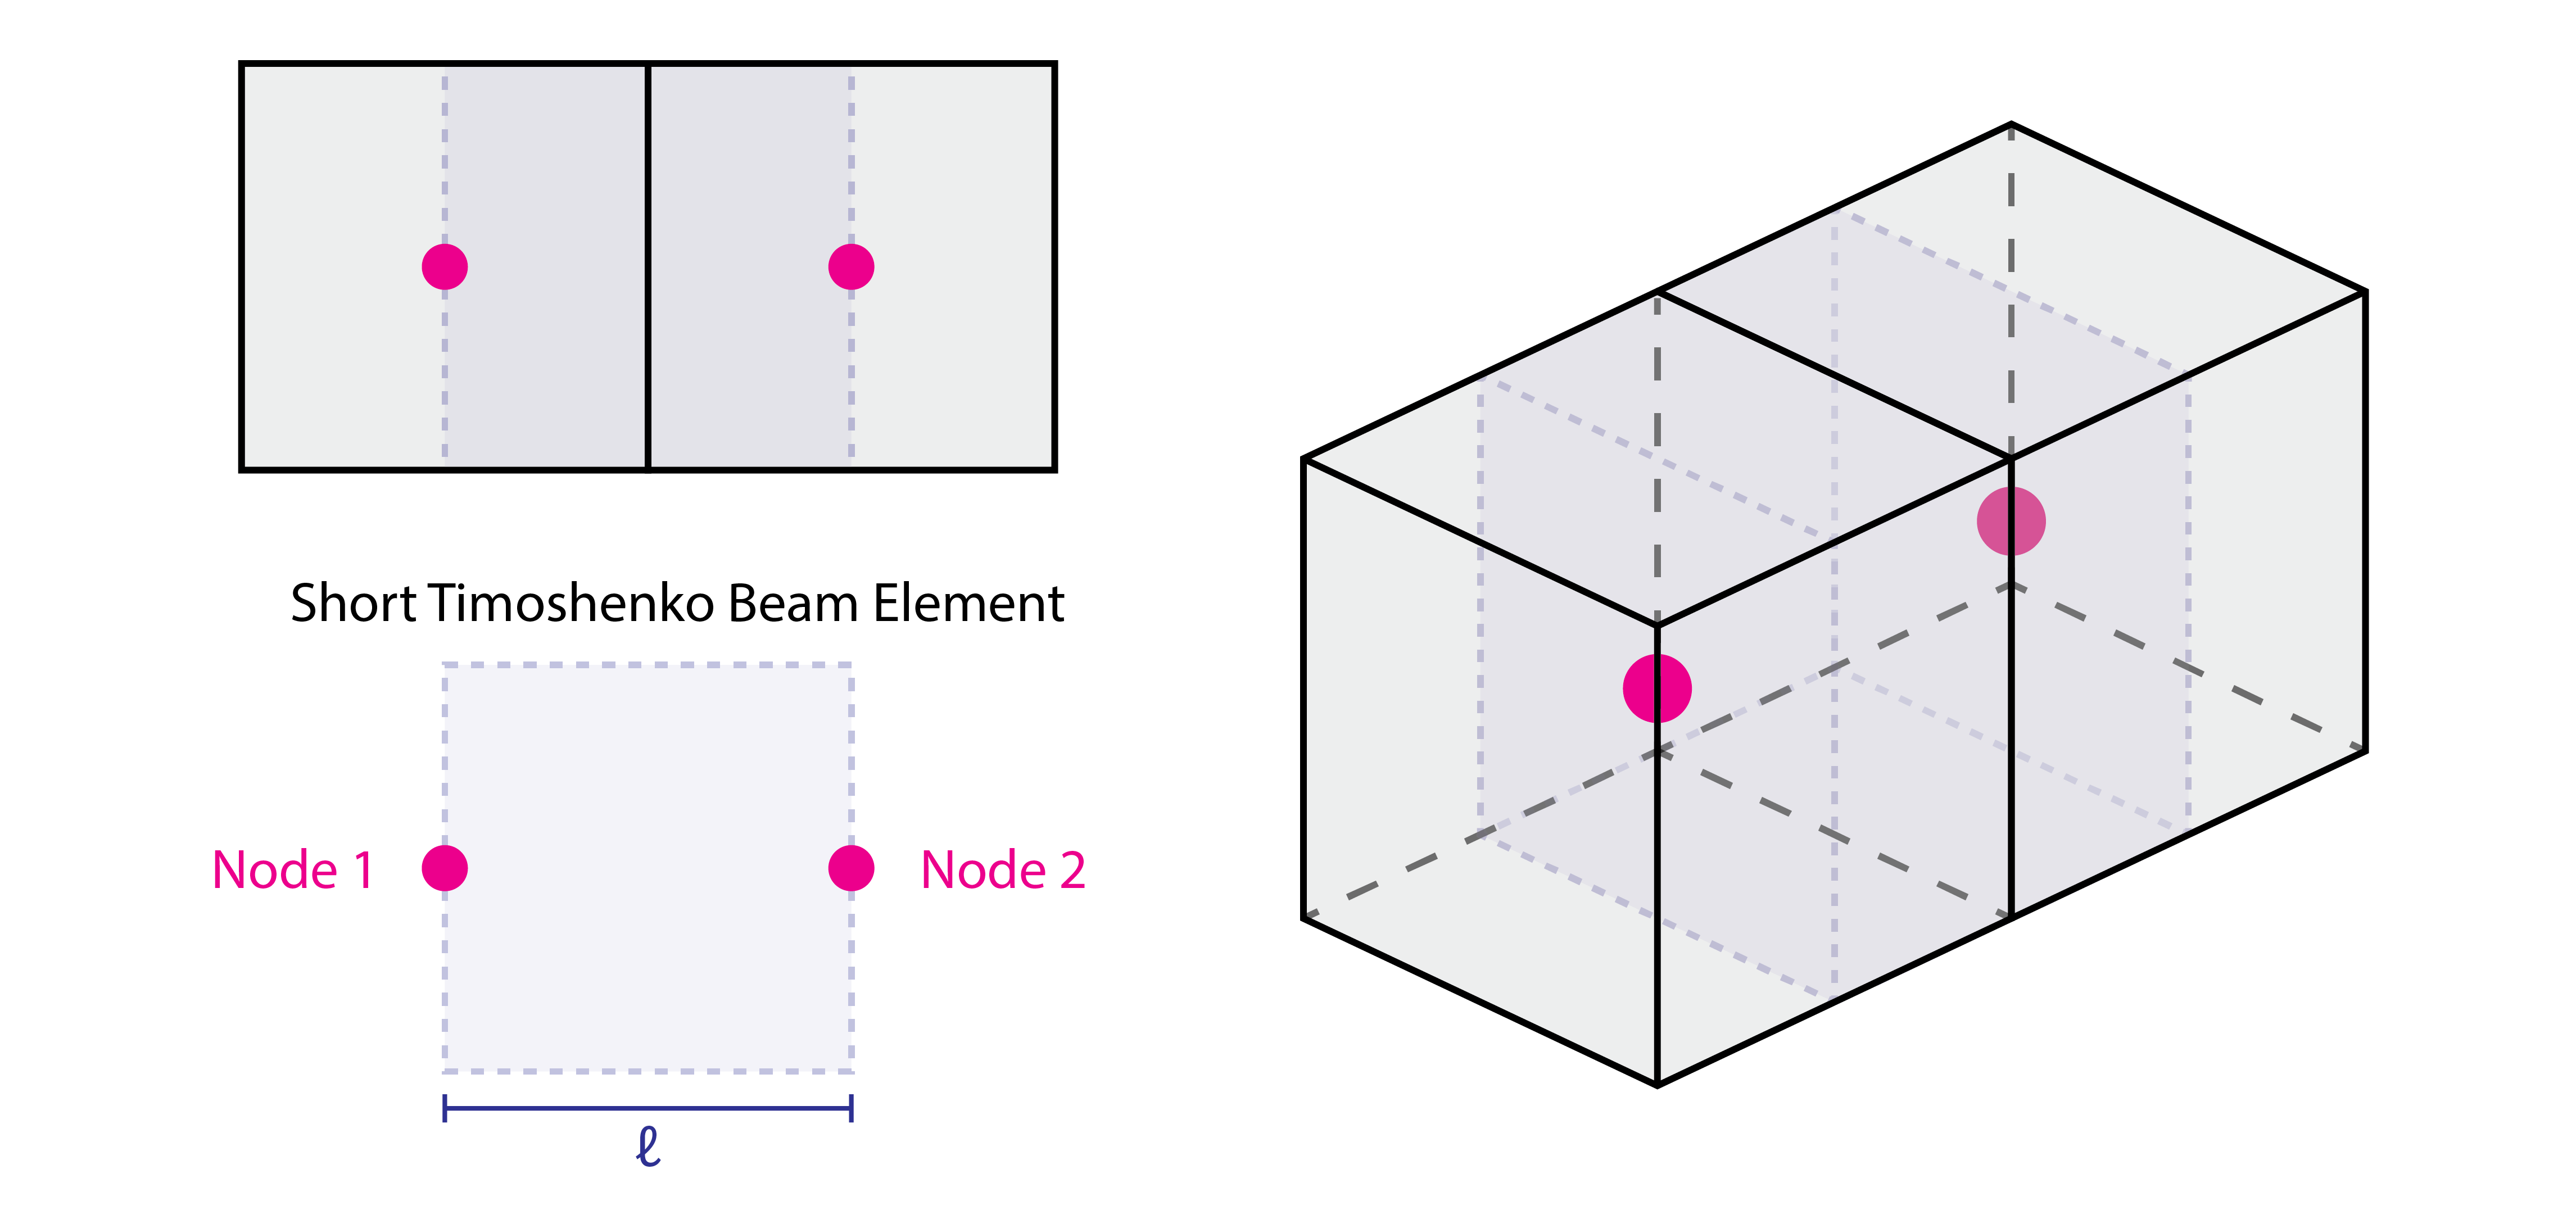
\includegraphics[width=\linewidth]{StubbyBeam.png}
  \caption{A diagram of the Timoshenko Beam Element joining two cells in my model.  Due to the low length and relatively high cross sectional area of this ``beam'', I argue that a shear-dominated Timoshenko beam is an appropriate model.}
  \label{fig:StubbyBeam}
\end{figure}

Some bending components of Equations \ref{eq:fy1}, \ref{eq:fz1}, \ref{eq:ty1}, \ref{eq:tz1}, \ref{eq:fy2}, \ref{eq:fz2}, \ref{eq:ty2},  and \ref{eq:tz2} are absent from the model described in Chapter \ref{chap:functionSim}.  Though the model still has a bending stiffness component, it is a special case of the 12DOF Timoshenko Beam Element where shearing dominates bending.  This is appropriate considering the aspect ratio of the beam that we are using to model the two cells.  As beams become shorter/thicker shearing dominates, and as beams become longer/thinner bending dominates \cite{Bower2009}.  If we are considering a perfectly cubic lattice, the length of the beam element that we can draw between two cells has a length equal to its height and width: the ``beam'' is a cube (Figure \ref{fig:StubbyBeam}).  According to Bower \cite{Bower2009} there is no known accurate approximate theory of short beams.

%Assuming  bending dominance, we can reduce Equation \ref{eq:Fy1decomp} to:
%\[ F_{y1} =  \dfrac{12EI_z}{l^3} (p_{y2} -p_{y1}) - \dfrac{6EI_z}{l^2}(\theta_{z1} + \theta_{z2})  \]
%\[ F_{y1} =  \dfrac{12EI_z}{l^3} (p_{y2} -p_{y1}) - \dfrac{12EI_z}{l^3}(l\theta_{avg})  \]
%\[ F_{y1} =  \dfrac{12EI_z}{l^3} (p_{y2} -p_{y1} - l\theta_{avg})  \]
%
%Assuming bending dominance, \ref{eq:Ty1decomp} reduces to:
%\[T_{y1} = - \dfrac{6EI_y}{l^2}(p_{z2}- p_{z1}) - \dfrac{2EI_y}{l}(2\theta_{y1}  + \theta_{y2})\]

\subsection{Conclusion}

\begin{figure}
  \includegraphics[width=\linewidth]{deformationangle.png}
  \caption{Large angular deflection of bending flexures in a small assembly of functional parts. \textit{Image Credit: Will Langford 2016}}
  \label{fig:deformationangle}
\end{figure}

The model I've developed (Chapter \ref{chap:functionSim}) for cell-cell interaction is similar to a shear-dominated 12DOF Timoshenko Beam Element joining the two cells.  Given the aspect ratio of the cells I am modeling, I argue that a shear-dominated beam model is appropriate.  The only difference between my model and a shear-dominated Timoshenko beam is that my model does not use any small angle approximations, and should therefore be more robust to large angular deformations between cells; we expect to see relatively large angular deformations in some of our parts (Figure \ref{fig:deformationangle}).

\section{Comparison with VoxCAD Physics Engine}

The model behind VoxCAD uses a special case of the 12DOF Timoshenko Beam Element called the Euler-Bernoulli Beam Element \cite{Hiller2014a}.  The Euler-Bernoulli model assumes no shearing of a beam element joining two cells - it is a bending-dominated form of Timoshenko.  For a beam oriented along the x-axis, using the same Hermitian cubic shape functions, we get the following stiffness matrix for an Euler-Bernoulli beam:

\[ K =  \small {\left[ \begin{smallmatrix}
\tfrac{EA}{l} & 0 & 0 & 0 & 0 & 0 & \tfrac{-EA}{l} & 0 & 0 & 0 & 0 & 0\\
 & \tfrac{12EI_z}{l^3} & 0 & 0 & 0 & \tfrac{6EI_z}{l^2} & 0 & \tfrac{-12EI_z}{l^3} & 0 & 0 & 0 & \tfrac{6EI_z}{l^2}\\
 &  & \tfrac{12EI_y}{l^3} & 0 & \tfrac{-6EI_y}{l^2} & 0 & 0 & 0 & \tfrac{-12EI_y}{l^3} & 0 & \tfrac{-6EI_y}{l^2} & 0\\
 &  &  &  \tfrac{GJ}{l} &  0 &  0 &  0 &  0 &  0 & \tfrac{-GJ}{l} & 0 & 0\\
 &  &  &  & \tfrac{4EI_y}{l} & 0 & 0 & 0 & \tfrac{6EI_y}{l^2} & 0 & \tfrac{2EI_y}{l} & 0\\
 &  &  &  &  & \tfrac{4EI_z}{l} & 0 & \tfrac{-6EI_z}{l^2} & 0 & 0 & 0 & \tfrac{2EI_z}{l}\\
 &  &  &  &  &  & \tfrac{EA}{l}  & 0 & 0 & 0 & 0 & 0\\
 &  &  &  &  &  &  & \tfrac{12EI_z}{l^3} & 0 & 0 & 0 & \tfrac{-6EI_z}{l^2}\\
 &  &  &  &  &  &  &  & \tfrac{12EI_y}{l^3} & 0 & \tfrac{6EI_y}{l^2}\ & 0\\
 &  & symmetric &  &  &  &  &  &  & \tfrac{GJ}{l} & 0 & 0\\
 &  &  &  &  &  &  &  &  &  & \tfrac{4EI_y}{l} & 0\\
  &  &  &  &  &  &  &  &  &  &  & \tfrac{4EI_z}{l}\\
 \end{smallmatrix} \right] } \]
 
 This is equivalent to the 12DOF Timoshenko stiffness matrix with the shear terms $\phi$ removed.  Multiplying through Equation \ref{eq:forcestiffnessdisp} gives us 12 equations:

\begin{subequations}
\begin{align} 
\label{eq:fx1vox}
F_{x1} &=  -\dfrac{EA}{l}p_{x1} + \dfrac{EA}{l}p_{x2} \\[10pt]
\label{eq:fy1vox}
F_{y1} &=  -\dfrac{12EI_z}{l^3}p_{y1} - \dfrac{6EI_z}{l^2}\theta_{z1} + \dfrac{12EI_z}{l^3}p_{y2} - \dfrac{6EI_z}{l^2}\theta_{z2}\\[10pt]
\label{eq:fz1vox}
F_{z1} &= - \dfrac{12EI_y}{l^3}p_{z1} + \dfrac{6EI_y}{l^2}\theta_{y1} + \dfrac{12EI_y}{l^3}p_{z2} + \dfrac{6EI_y}{l^2}\theta_{y2}\\[10pt]
\label{eq:tx1vox}
T_{x1} &=  -\dfrac{GJ}{l}\theta_{x1} + \dfrac{GJ}{l}\theta_{x2} \\[10pt]
\label{eq:ty1vox}
T_{y1} &= \dfrac{6EI_y}{l^2}p_{z1} - \dfrac{4EI_y}{l}\theta_{y1}  - \dfrac{6EI_y}{l^2}p_{z2} - \dfrac{2EI_y}{l}\theta_{y2} \\[10pt]
\label{eq:tz1vox}
T_{z1} &=  -\dfrac{6EI_z}{l^2}p_{y1} - \dfrac{4EI_z}{l}\theta_{z1}  + \dfrac{6EI_z}{l^2}p_{y2} - \dfrac{2EI_z}{l}\theta_{z2} \\[10pt]
\label{eq:fx2vox}
F_{x2} &=  -F_{x1}\\[10pt]
\label{eq:fy2vox}
F_{y2} &=  -F_{y1}\\[10pt]
\label{eq:fz2vox}
F_{z2} &=  -F_{z1}\\[10pt]
\label{eq:tx2vox}
T_{x2} &=  -T_{x1}\\[10pt]
\label{eq:ty2vox}
T_{y2} &=  \dfrac{6EI_y}{l^2}p_{z1} - \dfrac{2EI_y}{l}\theta_{y1}  - \dfrac{6EI_y}{l^2}p_{z2} - \dfrac{4EI_y}{l}\theta_{y2} \\[10pt]
\label{eq:tz2vox}
T_{z2} &= -\dfrac{6EI_z}{l^2}p_{y1} - \dfrac{2EI_z}{l}\theta_{z1}  + \dfrac{6EI_z}{l^2}p_{y2} - \dfrac{4EI_z}{l}\theta_{z2}
\end{align}
\end{subequations}\\

\subsection{Conclusion}

As I described in Section \ref{sec:bendingdominance}, a bending dominated beam model is more appropriate for long, thin beams.   Given the aspect ratio of the elements being modeled in VoxCAD (very similar to what I've been modeling), the absence of shearing likely causes deflections to be underestimated \cite{Bower2009}.  Additionally, VoxCAD relies on the same small angle approximations present in the Timoshenko model.\\

That being said, my model draws enormous inspiration from VoxCAD, specifically in the handling of composite stiffness and damping constants for multimaterial junctions (Equations \ref{eq:springseries}, \ref{eq:damperseries}), calculation of maximum time step $\Delta t$ (Equations \ref{eq:maxnatFreq} and \ref{eq:maxDeltaT}), and translational actuation model.  Furthermore, seeing the performance that VoxCAD was able to achieve made me more confident to embark on this work in the first place. 

\section{Comparison with COMSOL Simulation}

\begin{figure}
  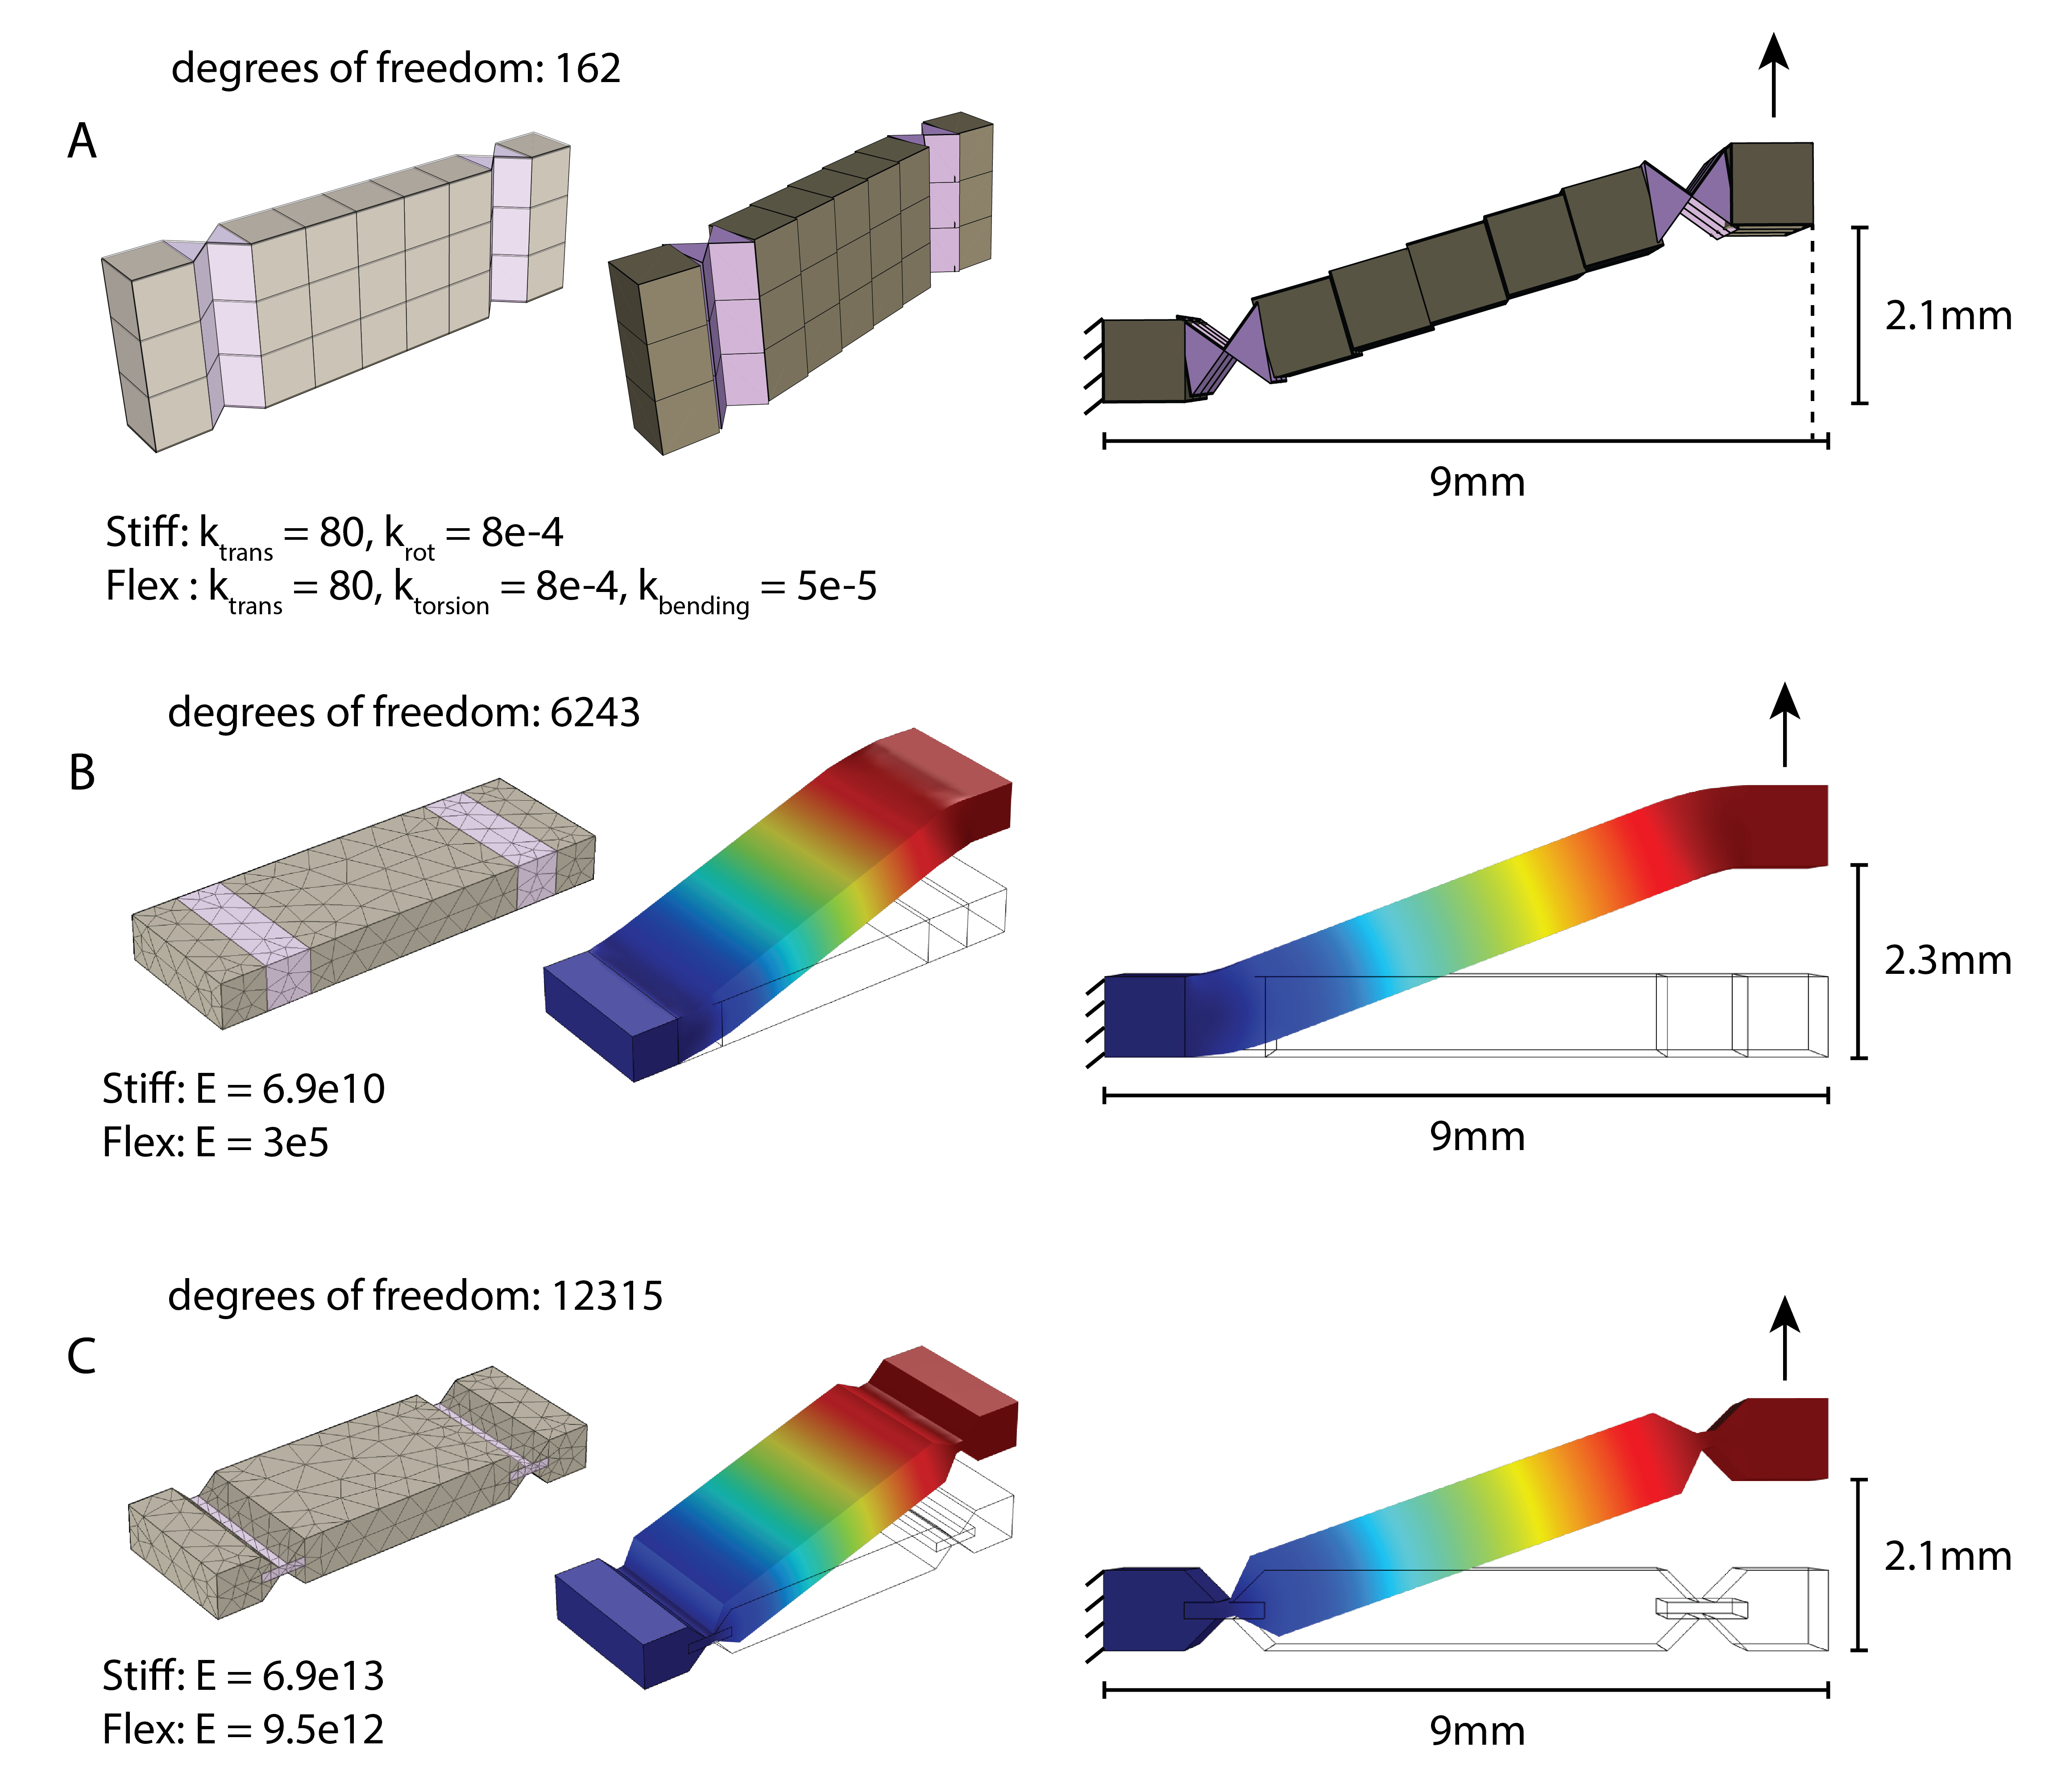
\includegraphics[width=\linewidth]{somsolsim1.png}
  \caption{Simulation of a shear flexure functional part in TBD \textbf{(A)} and in COMSOL using a simple geometric model \textbf{(B)} and a more detailed model \textbf{(C)}.  Real parts shown in Figure \ref{fig:deformationangle}.  Note - the special meshes used for the 1DOF bending flexures in \textbf{A} are meant for visualization only, the underlying geometry is assumed to be identical to \textbf{B}.}
  \label{fig:somsolsim1}
\end{figure}

In simulation we wish to represent functional primitives as geometrically simple elements with isotropic and anisotropic material properties deriving from their internal structure.  This way we can discretize them with a relatively low resolution mesh and increase the efficiency of the simulation.  I started by using the same geometric representation I'm using in my model, shown in Figure \ref{fig:somsolsim1}B. Using this minimal geometry, I had trouble decoupling bending and axial stiffness (explained in Section \ref{sec:decoupling}), so I switched to a more geometrically detailed model, shown in Figure \ref{fig:somsolsim1}C.\\

\begin{figure}
  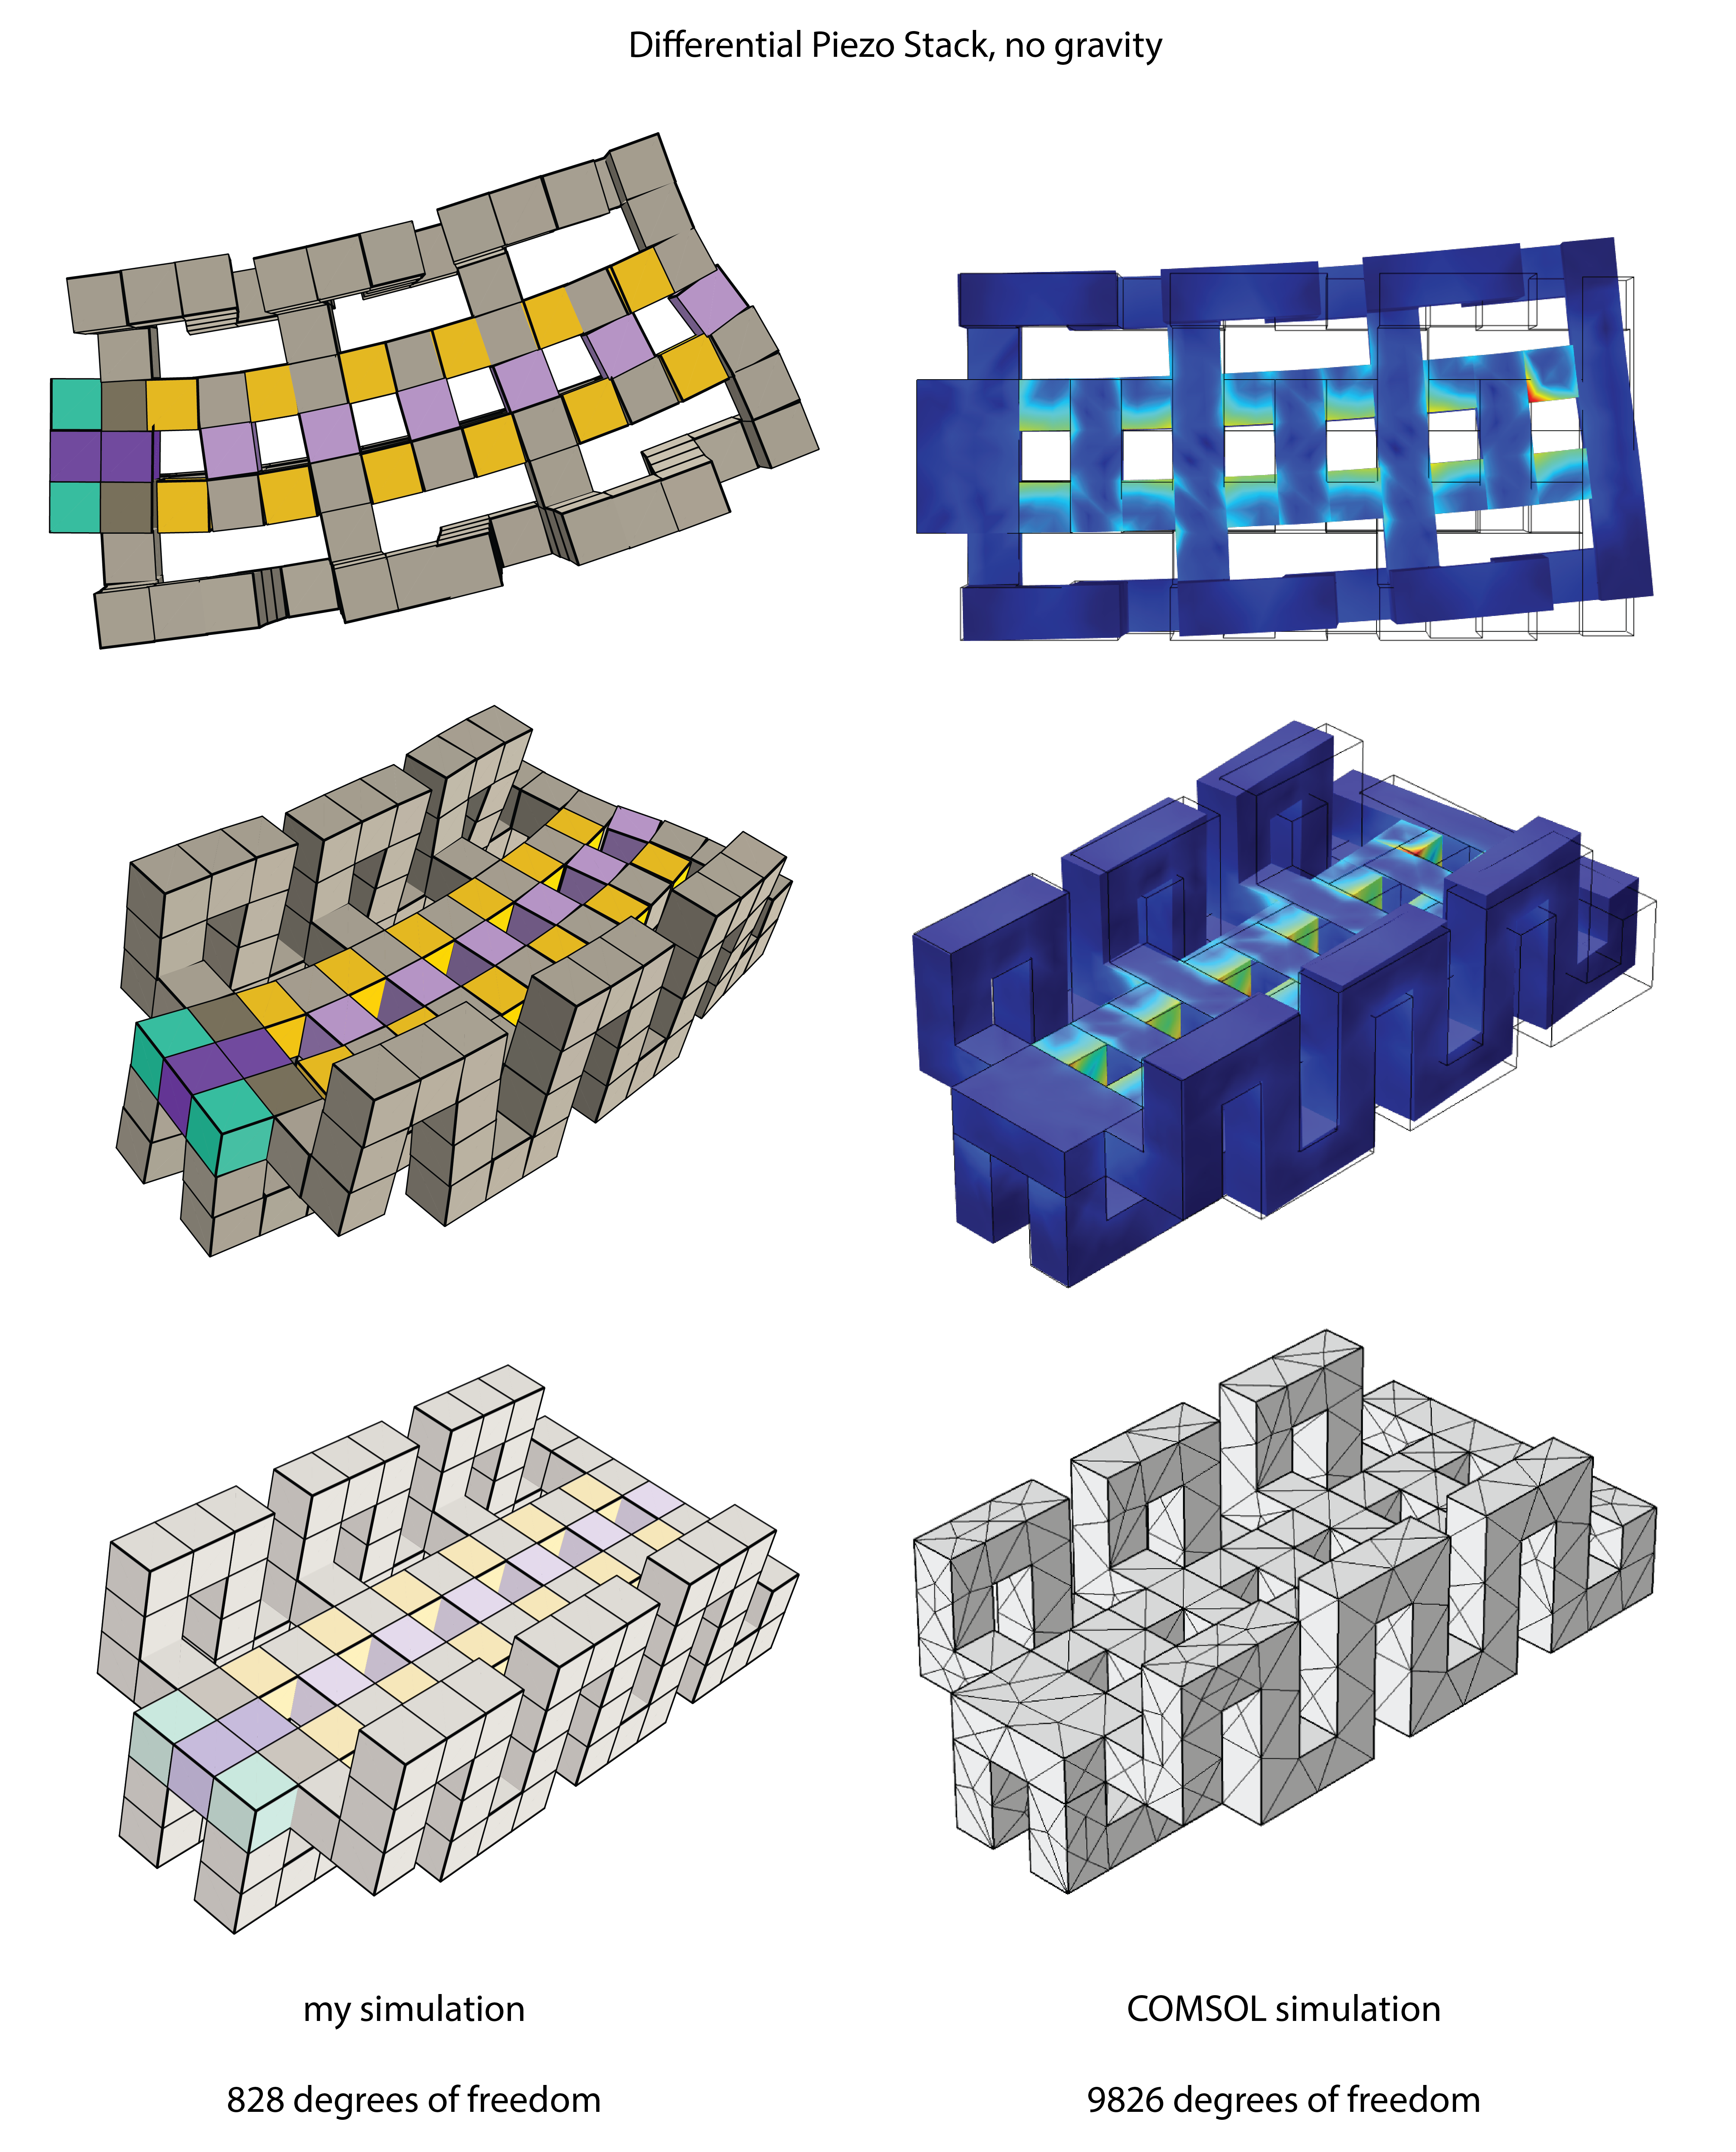
\includegraphics[width=\linewidth]{bendySim.png}
  \caption{}
  \label{fig:bendSim}
\end{figure}

%\begin{figure}
%  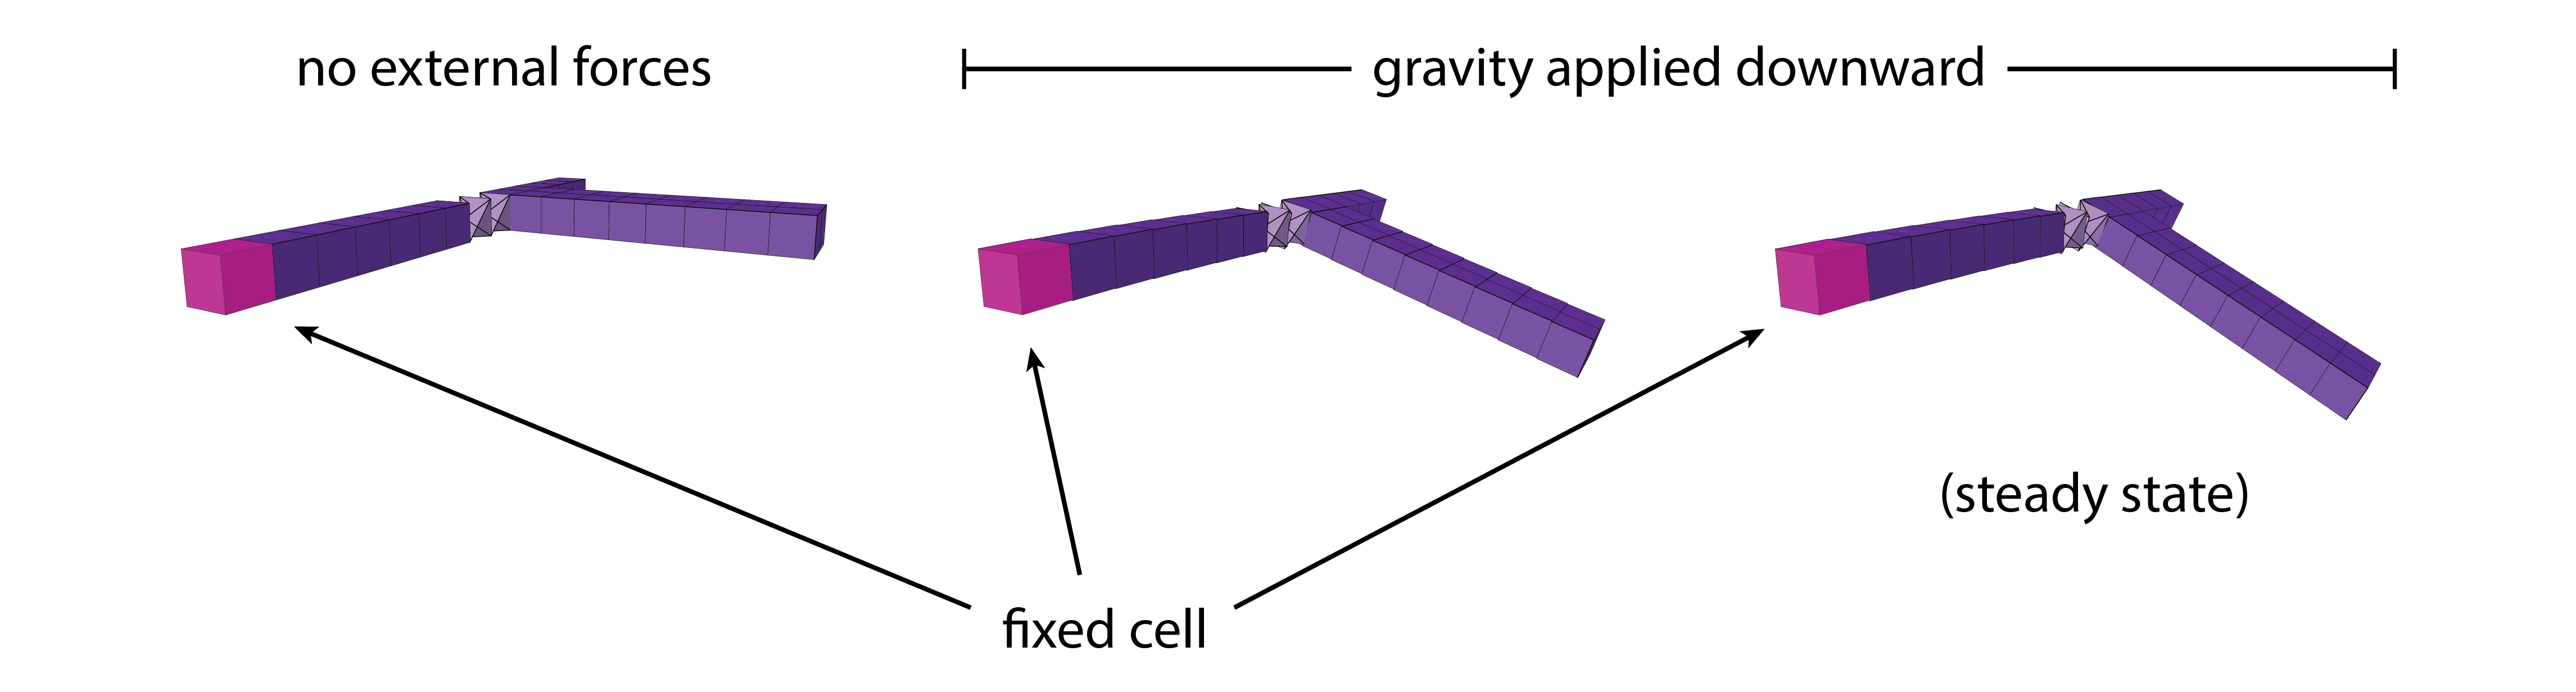
\includegraphics[width=\linewidth]{TorsionSim.png}
%  \caption{Qualitative simulation of a torsional flexure under a downward force from gravity shows appropriate anisotropic behavior.  Pink cell is fixed.}
%  \label{fig:TorsionSim}
%\end{figure}

\subsection{Conclusion}

%\begin{figure}
%  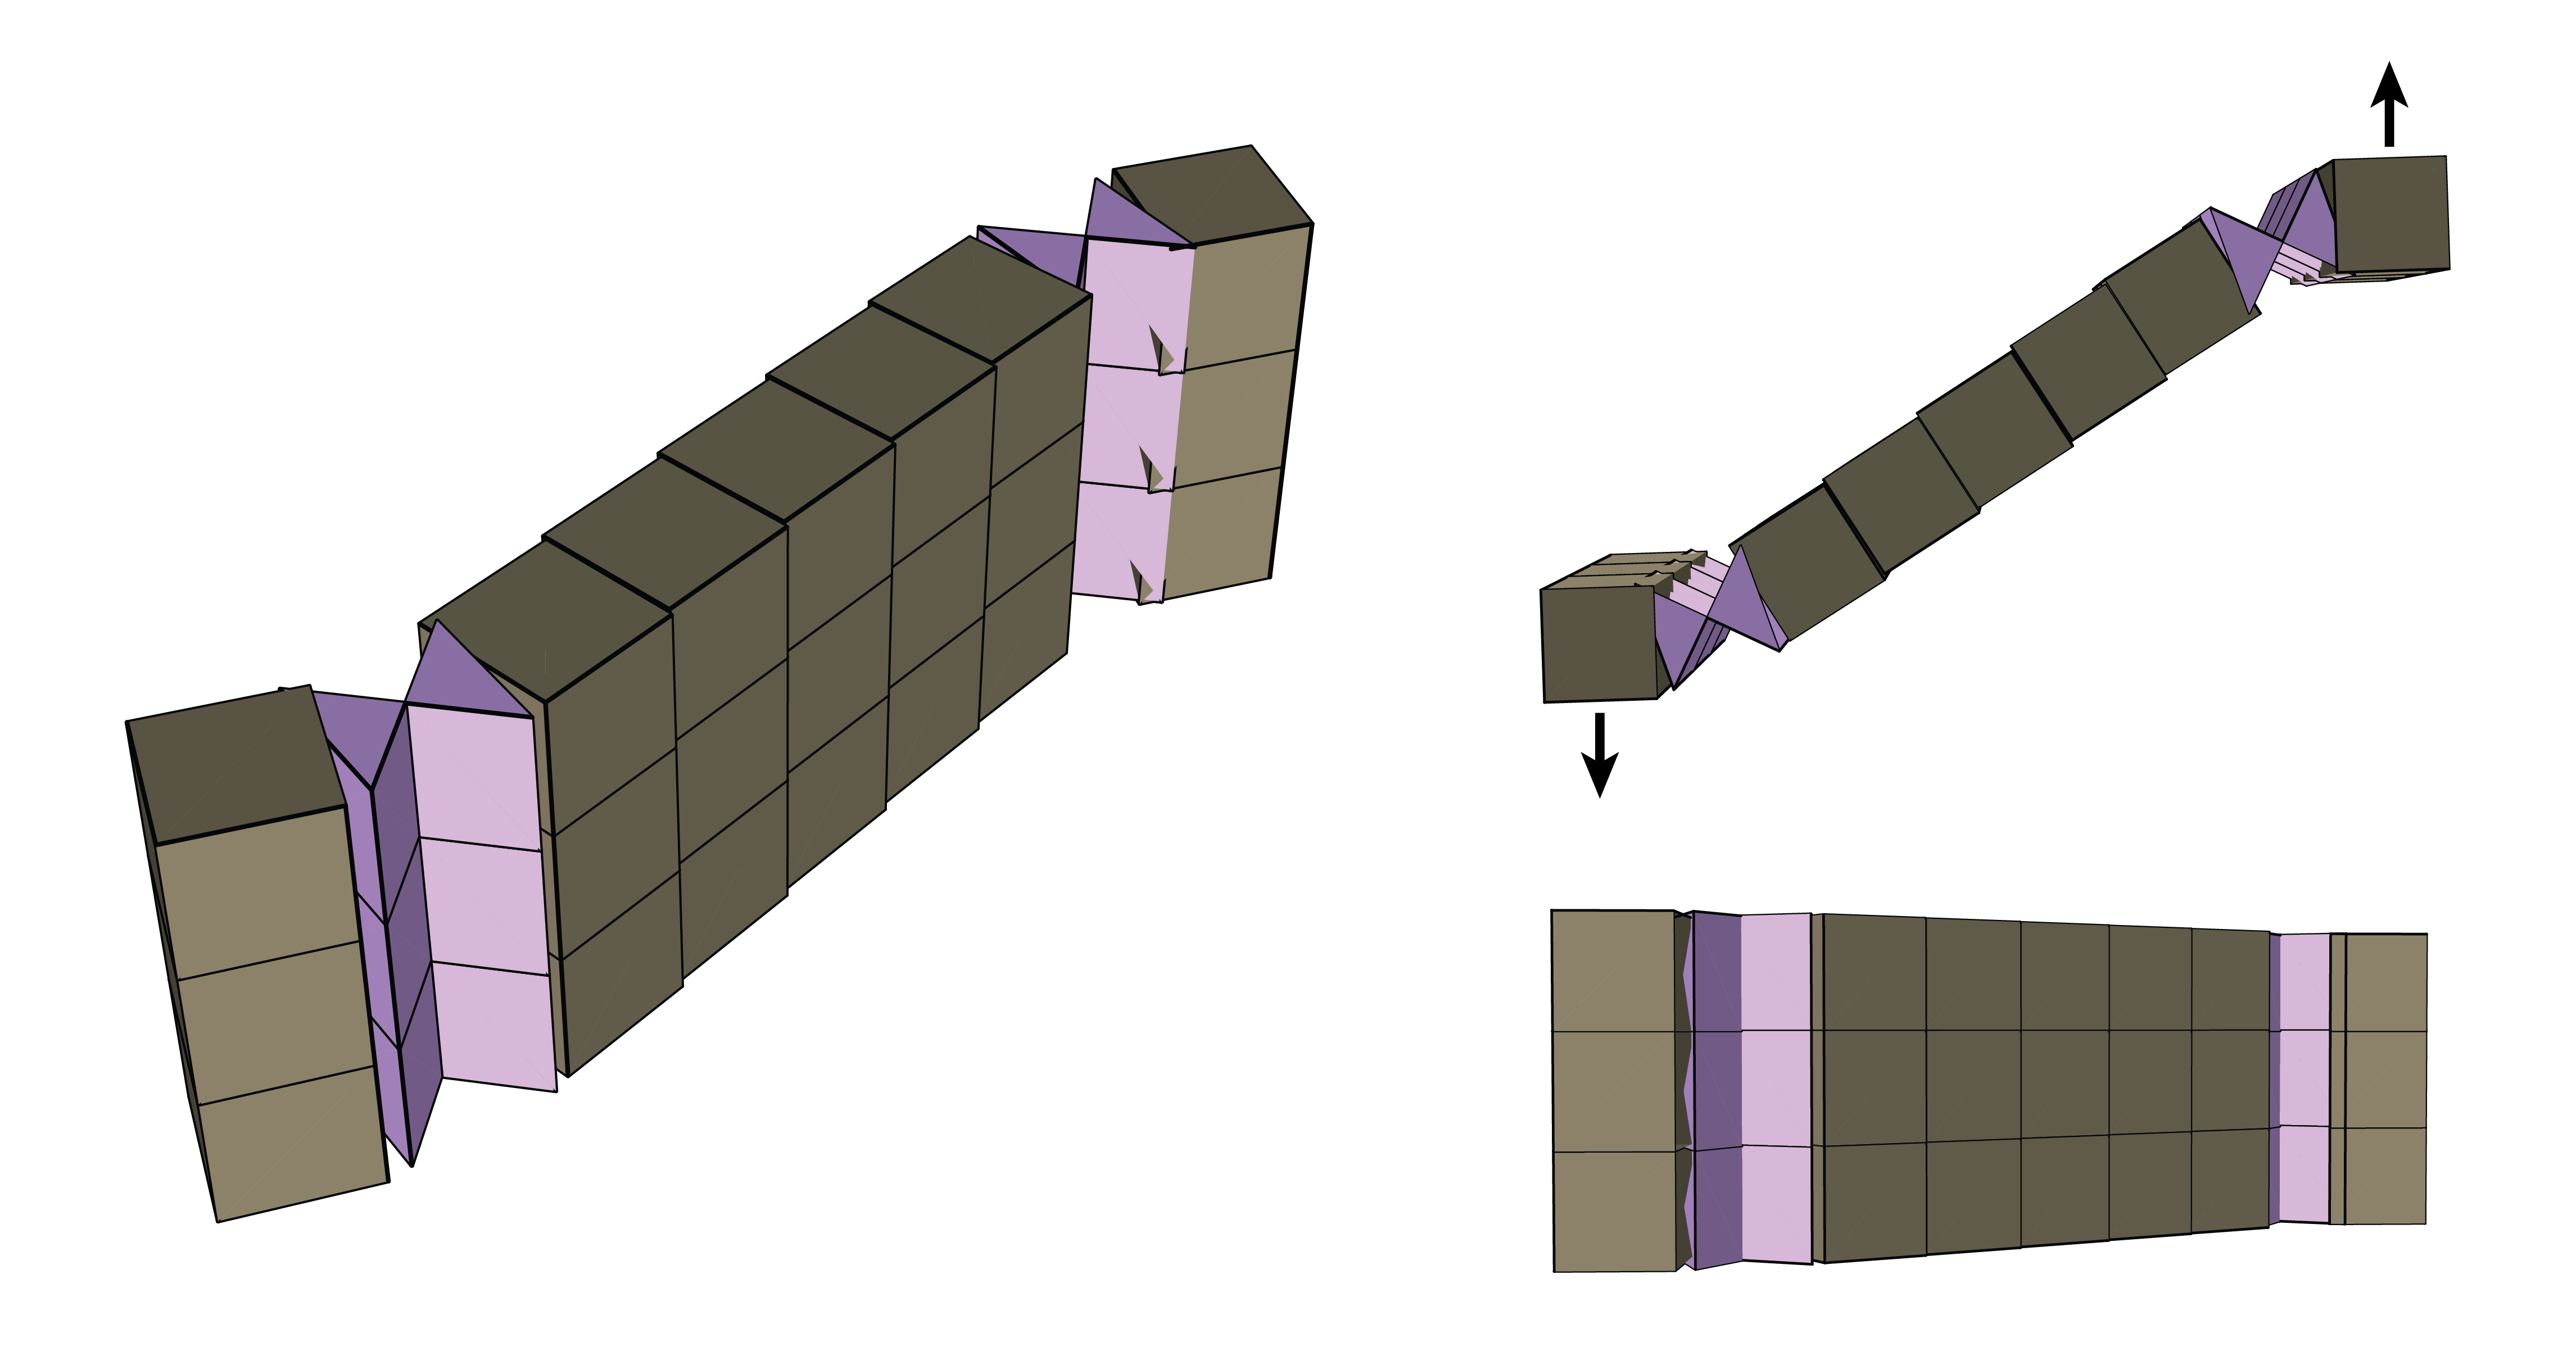
\includegraphics[width=\linewidth]{shearpart.png}
%  \caption{Qualitative simulation of shear flexure functional part from Figure \ref{fig:deformationangle} shows similar behavior in response to applied forces.}
%  \label{fig:shearpart}
%\end{figure}

The current state of my software implementation does not allow me to do a quantitative analysis of the model developed Chapter \ref{chap:functionSim} (debugging needed), but it does appear to be giving the correct qualitative behavior in the example shown in Figure \ref{fig:somsolsim1}A.

\subsubsection{Decoupling Axial/Bending and Shear/Torsion}\label{sec:decoupling}

Axial and bending stiffness typically use the same elastic modulus ($E$) in their formulations (Equations \ref{eq:kaxial} and \ref{eq:kbending}) and are therefore coupled to each other (e.g. you can't pick a value of $E$ that gives low bending stiffness and high axial stiffness at the same time for simple cubic geometry).  However, some composite materials exhibit these behaviors - Calisch showed that it is possible to build a structure that is stiff in axial compression and flexible in bending around one axis from four part types \cite{Calisch2014}.  This DOF coupling applies similarly to shear and torsional stiffness sharing the same shear stiffness $G$ (Equations \ref{eq:kshear} and \ref{eq:ktorsion}).  If we are trying to model a functional primitive that has complex internal geometric structure, we may need to decouple these degrees of freedom.\\

The only way to do this in COMSOL is to derive your own custom stiffness matrix for each of the anisotropic parts you wish to model or explicitly model their anisotropic geometries.  Defining your own stiffness matrix for each of these cell types requires a high degree of technical knowledge from the end user and essentially defeats the purpose of using a professional package; at that point you might as well write your own solver (essentially the situation I'm in).  Building a model of the substructures of each anisotropic cell type requires setting up even more material properties, geometries, and finer meshing of the model - slower from a user perspective and slower computationally.

\section{Performance Metrics}

\begin{figure}
  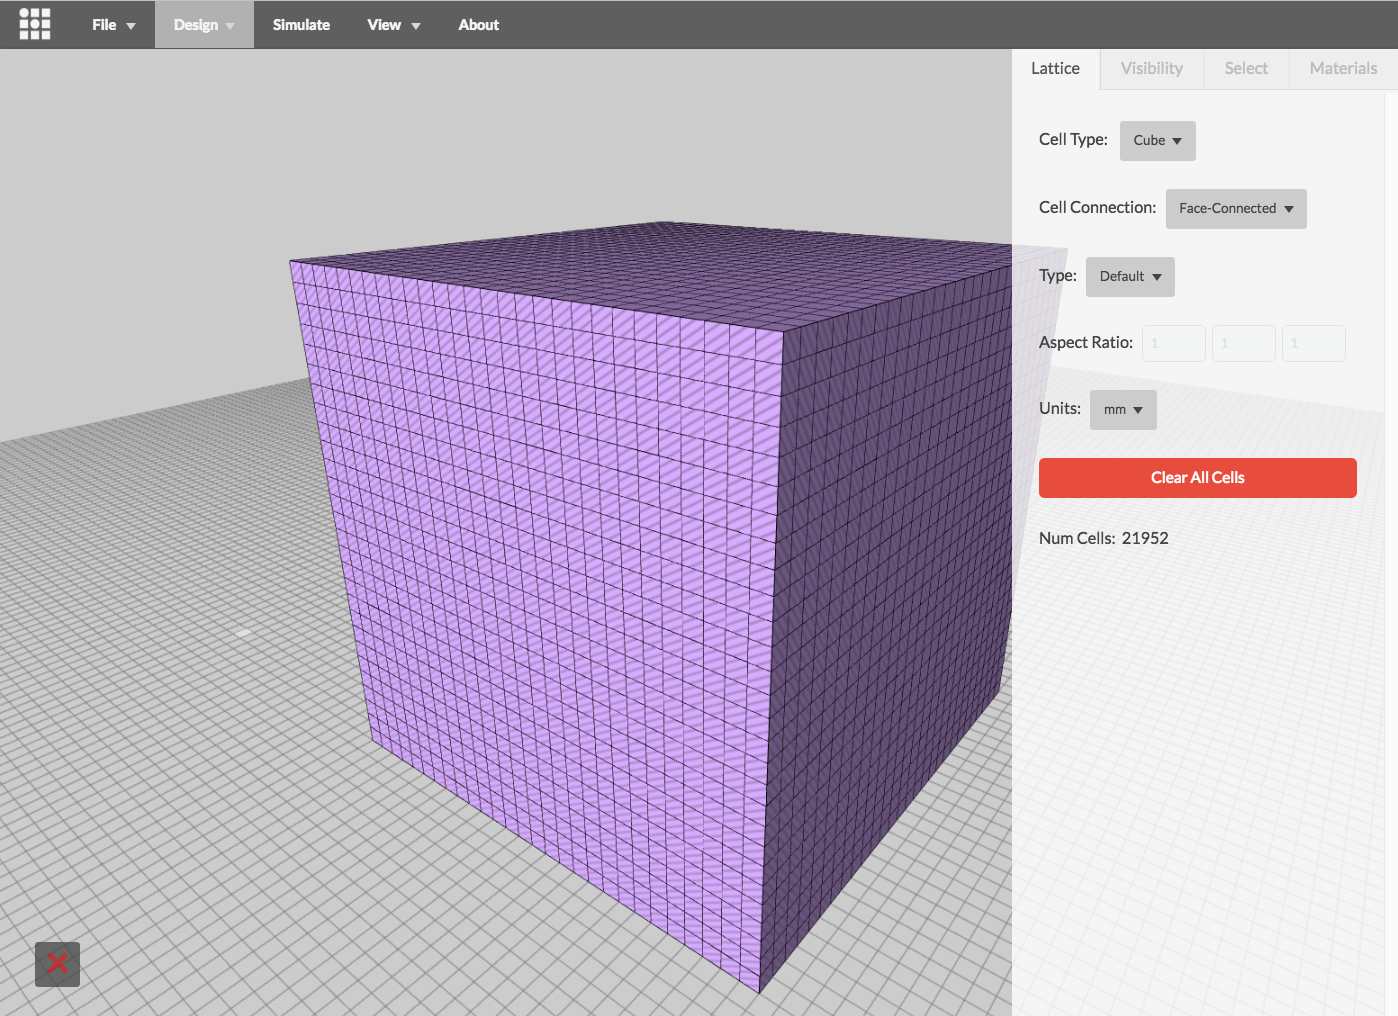
\includegraphics[width=\linewidth]{somanycells.png}
  \caption{A 28x28x28 cube containing 21952 cells.}
  \label{fig:somanycells}
\end{figure}

I performed a series of measurements to get a better understanding of where time was being spent during each complete render cycle of the simulation (simulation + threejs rendering).  I performed these tests on assemblies ranging from 1 cell to 21952 cells.  Since the amount of operations per simulation steps is proportional to the number of connections between cells, I ran these tests on cube-shaped assemblies (Figure \ref{fig:somanycells}), so the inner cells are all fully connected to their six neighbors.  This represents a ``worst case scenario'' performance-wise because cells are maximally connected, assemblies we will typically be modeling will not be as dense.  Smaller assemblies have the extra advantage that they have a greater surface area to volume ratio and are therefor proportionally more sparsely connected than larger assemblies of cells, but these effects drop off quickly.\\

I ran these tests using a AMD Radeon HD 6490M graphics card with 160 cores, clocked somewhere between 700-800MHz.  I set the threejs rendering window size to 1200x650px on a 1440x900px monitor and zoomed out so that all blocks were displayed in the rendering window.  Assemblies ranged in size from 1x1x1 to 28x28x28, or 21,952 cells.\\

\begin{figure}
  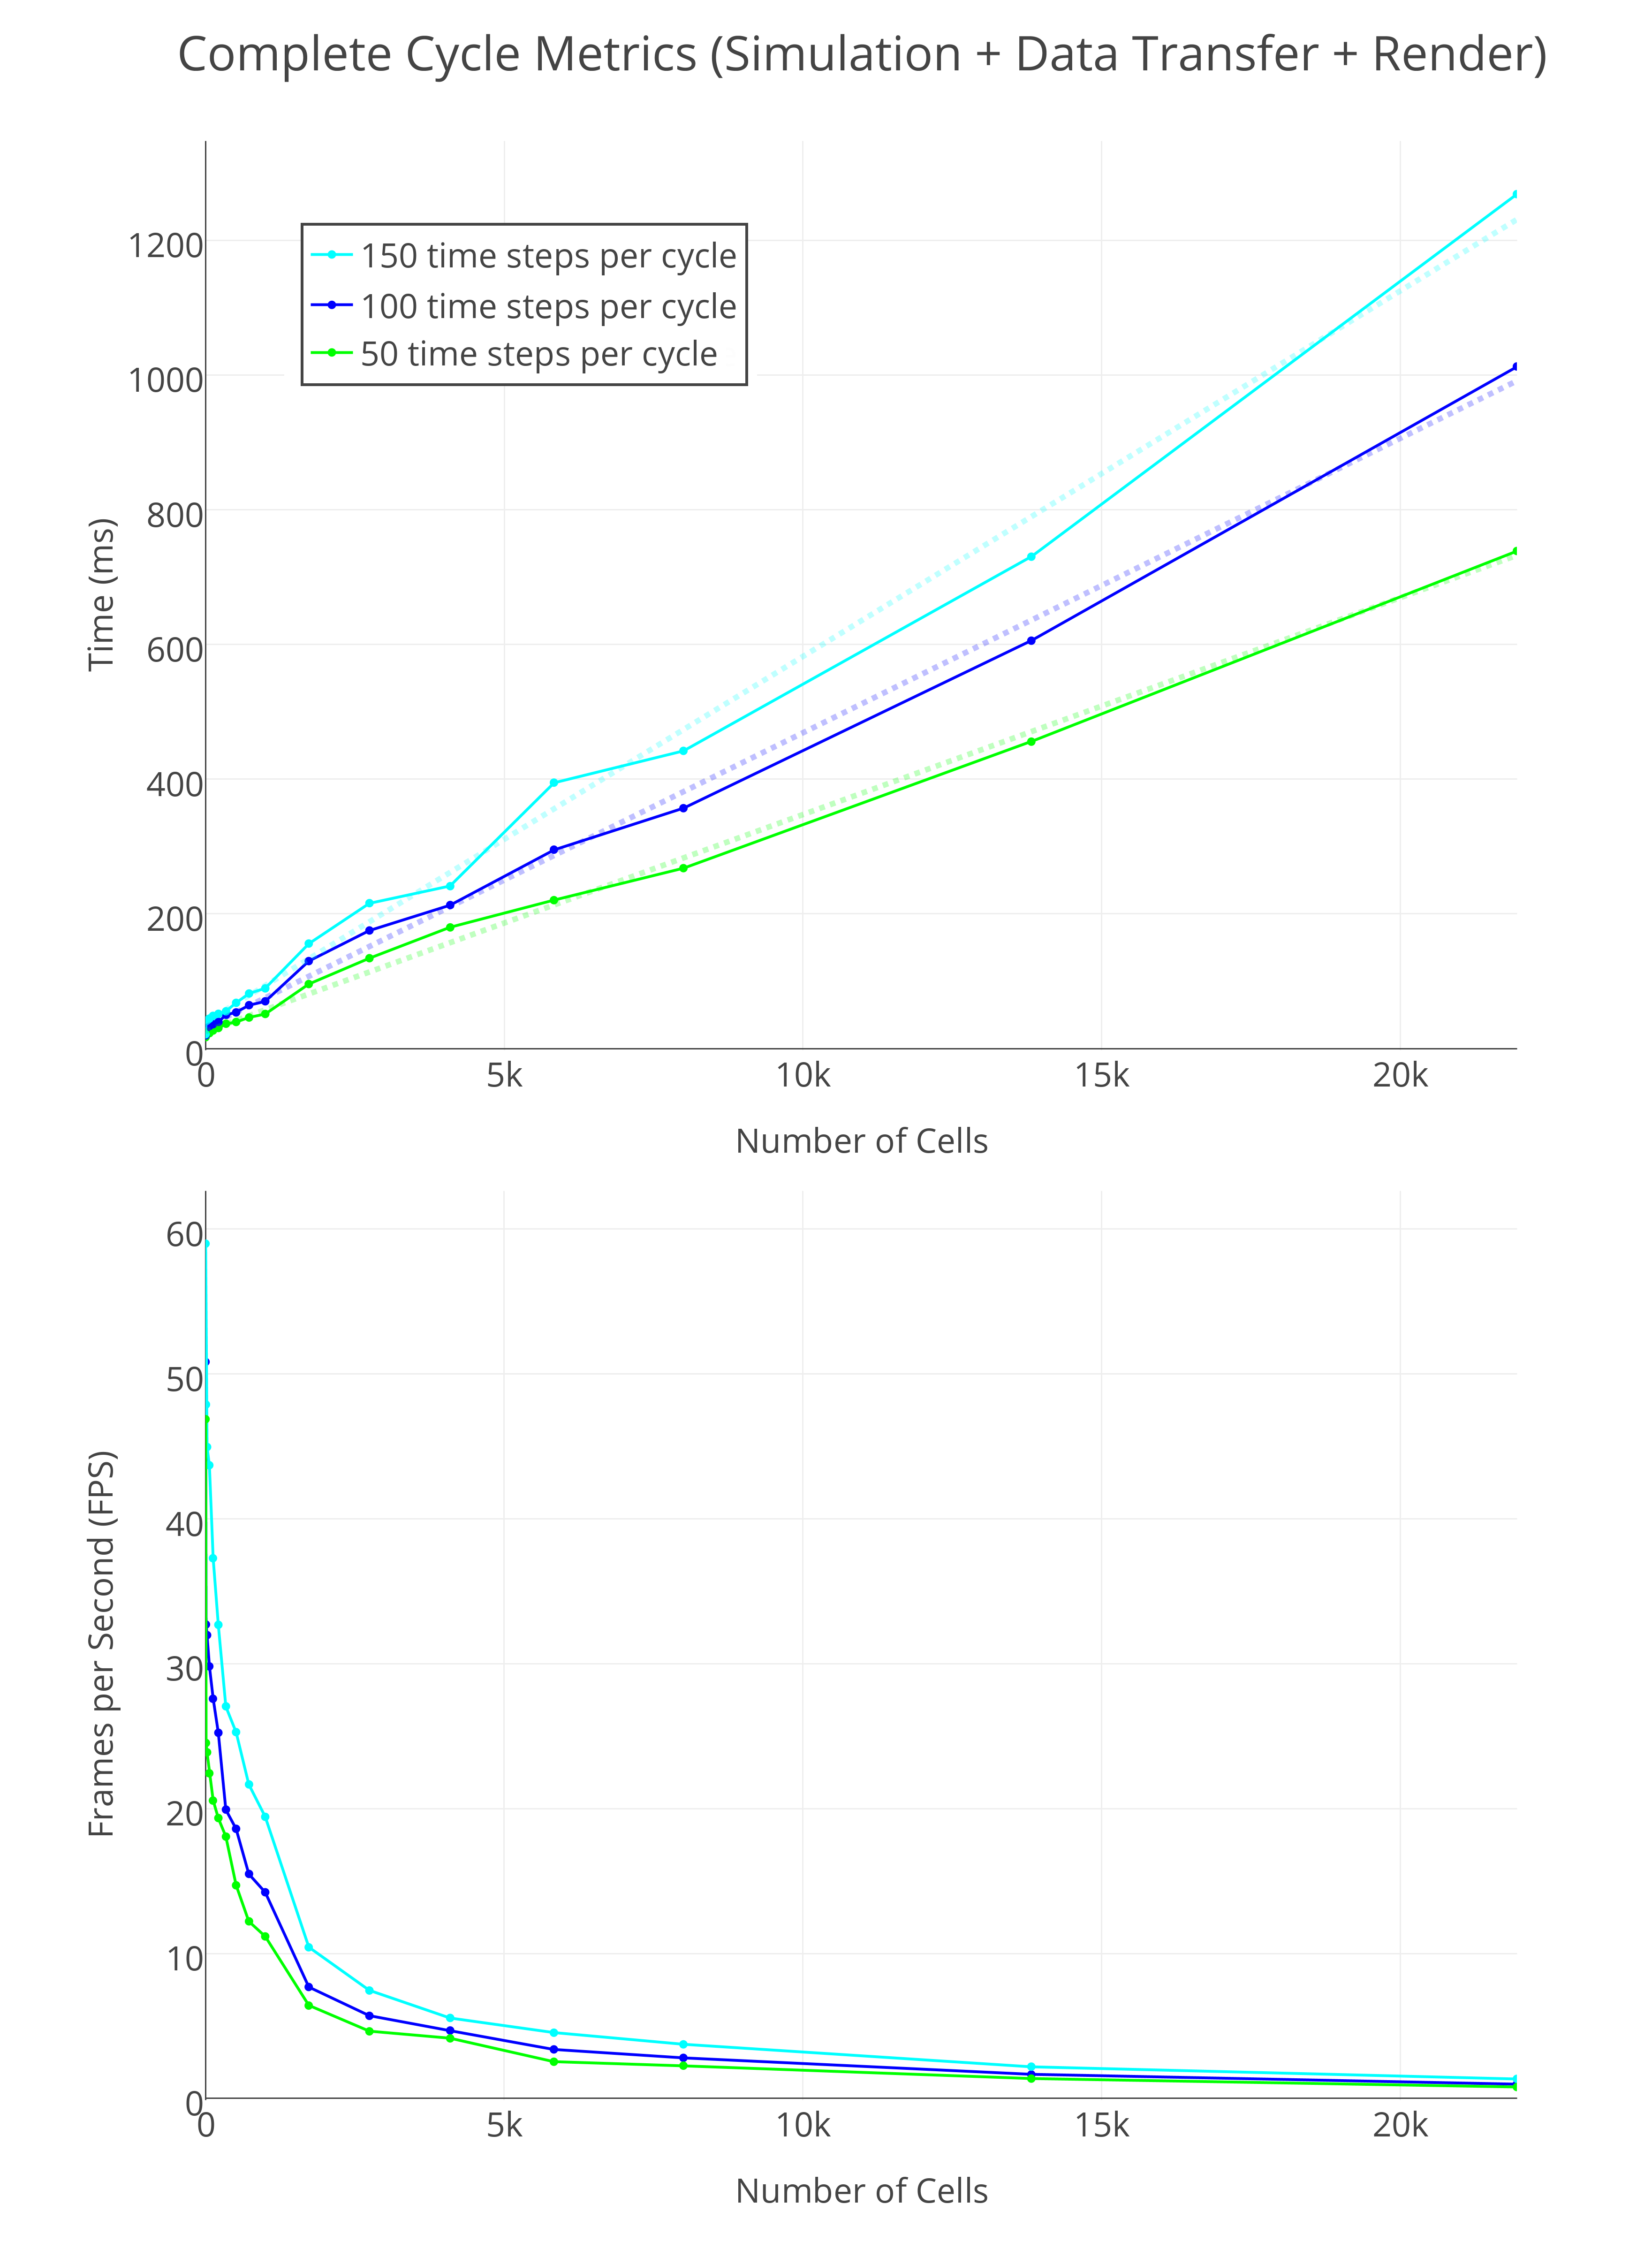
\includegraphics[width=\linewidth]{Metrics1.png}
  \caption{Render cycle speed shown in ms (top) and in FPS (bottom) for a series of assemblies spanning dimensions 1x1x1 to 28x28x28.  The number of simulation time steps solved per cycle was varied: 50 time steps (green), 100 time steps (navy), and 150 time steps (light blue). Linear fits to top plot shown with dotted lines.}
  \label{fig:Metrics1}
\end{figure}

Each complete render cycle consists of 3 stages: simulation, data transfer, and rendering.  The length of the simulation stage depends on the number of time steps that are being solved in the current render cycle.  Figure \ref{fig:Metrics1} shows plots for 50, 100, and 150 steps per cycle.  The data transfer stage is when the data from the final time step of simulation is pulled off the GPU and onto the CPU.  The rendering stage is when a render call is sent to threejs and graphics are rendered to the screen.

\subsection{Conclusions}

\begin{figure}
  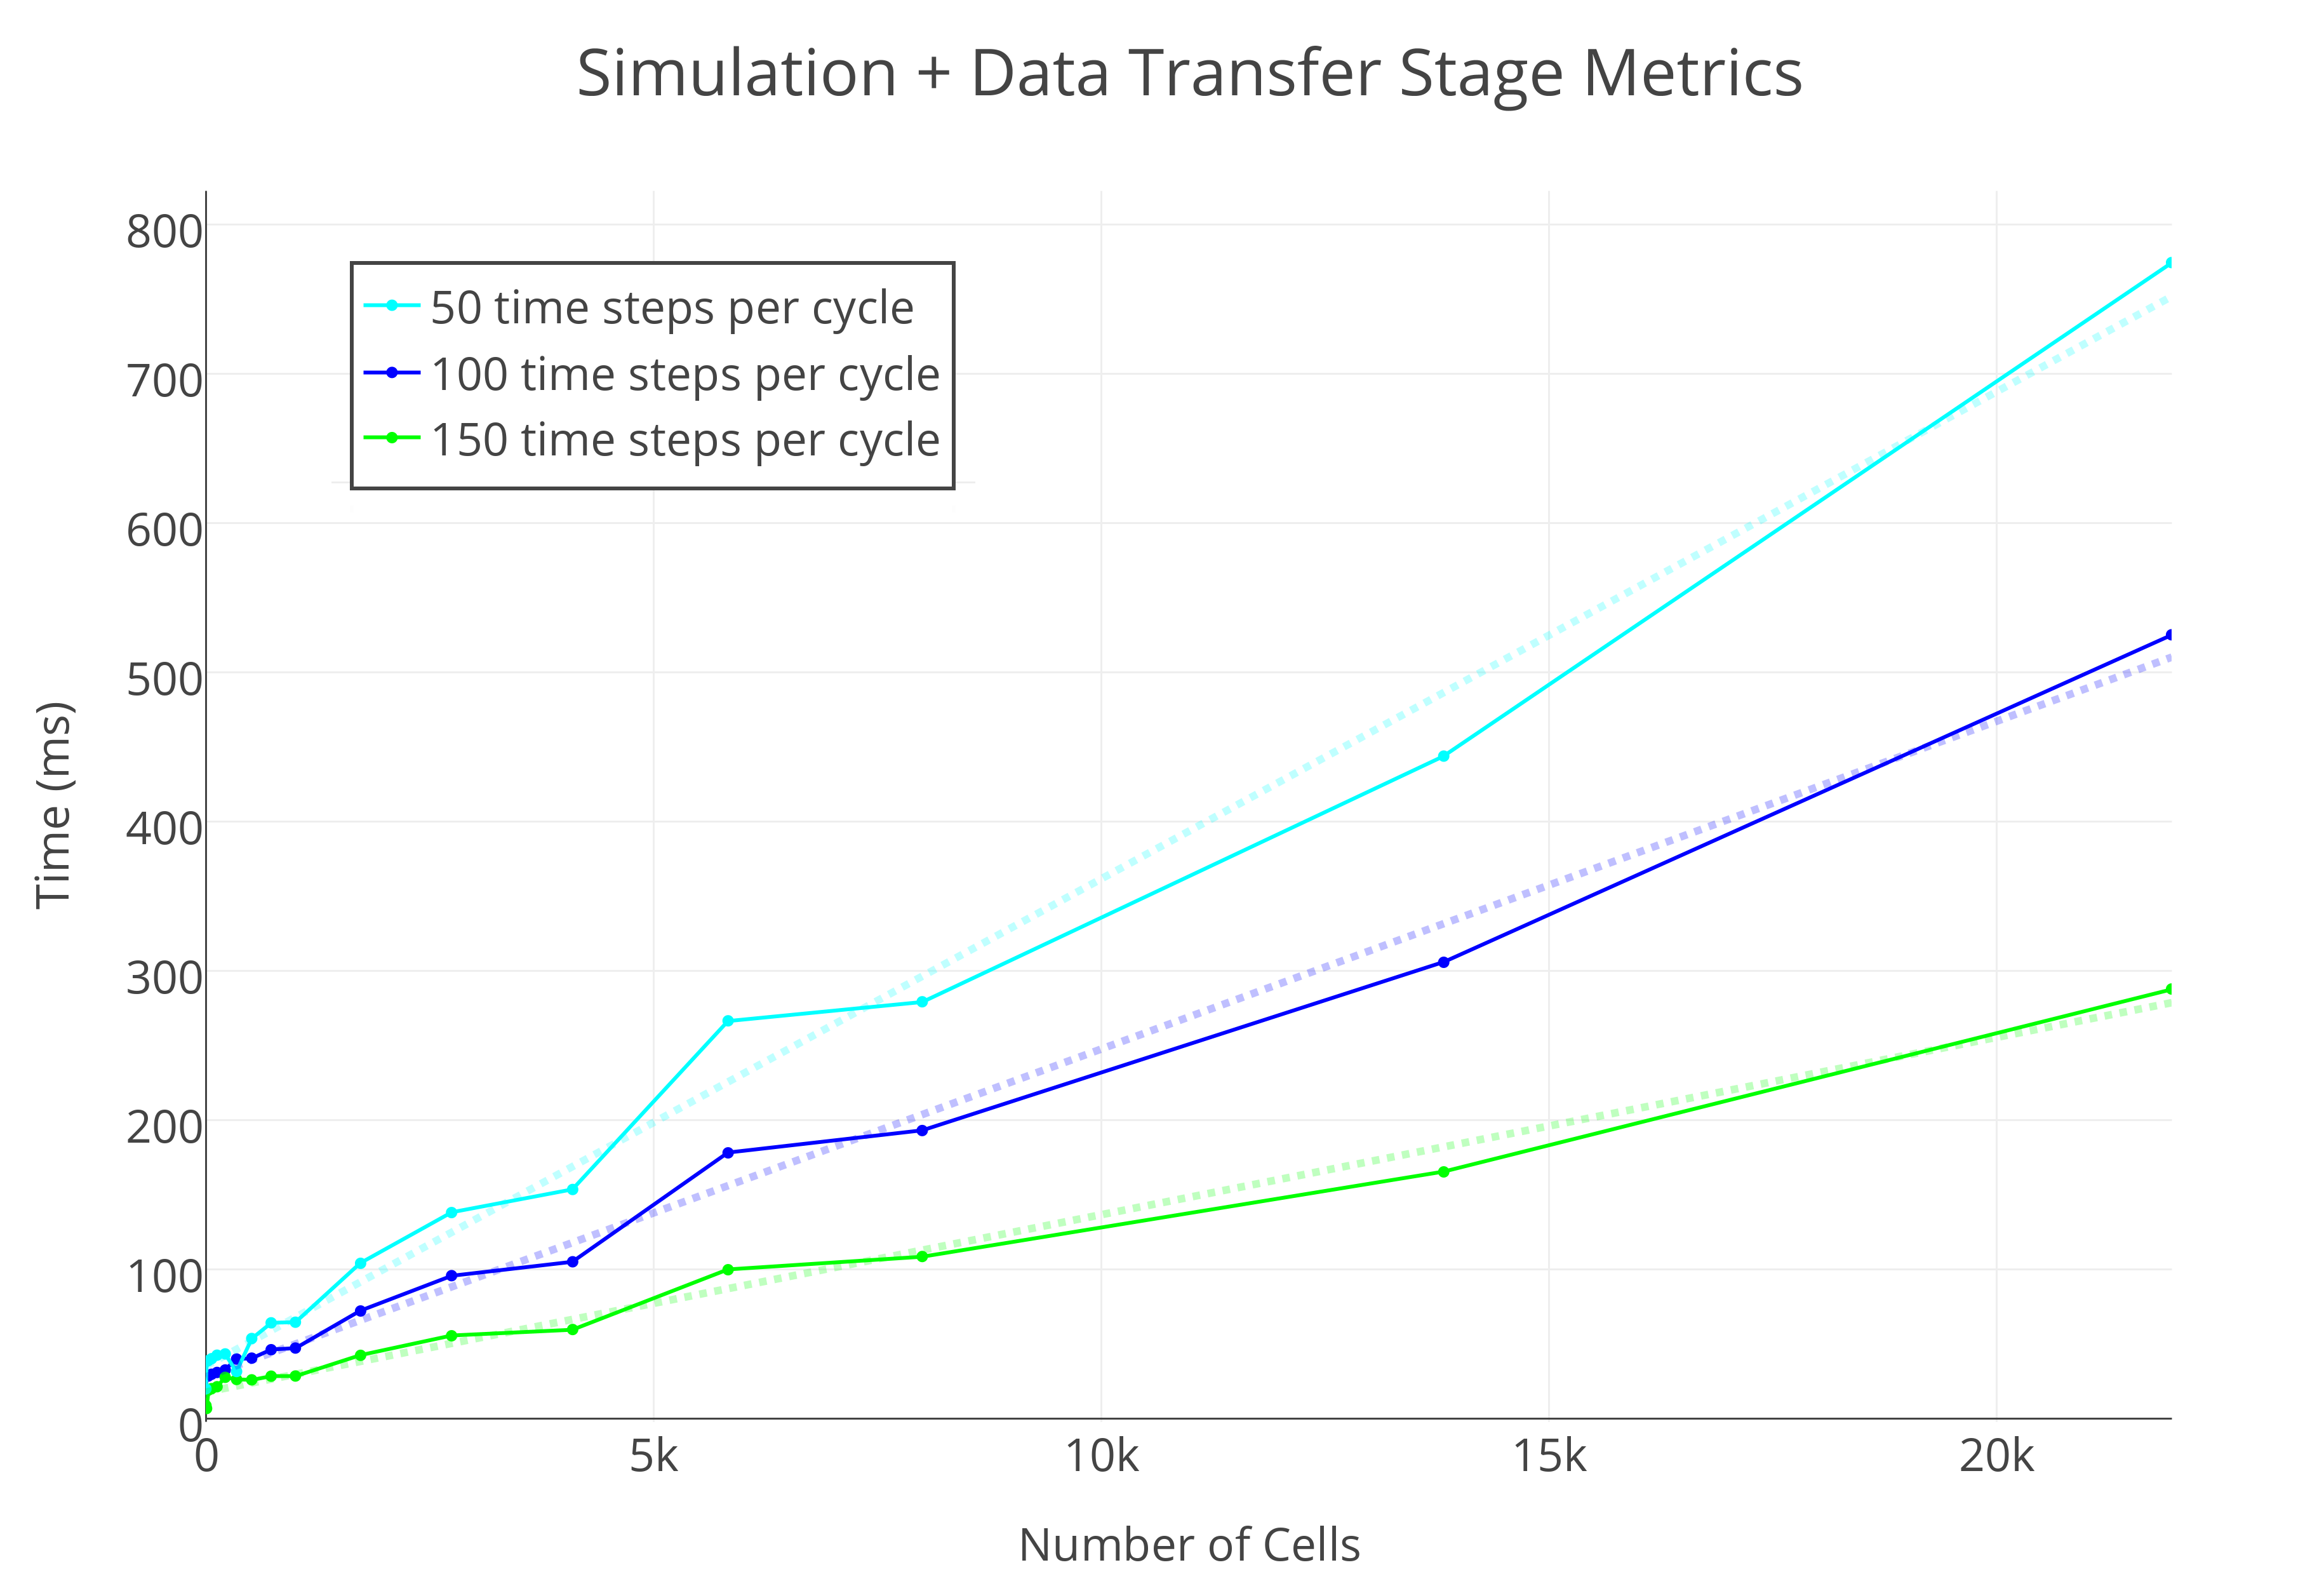
\includegraphics[width=\linewidth]{simdatatransmetrics.png}
  \caption{Duration of simulation and data transfer stages plotted for 50 time steps (green), 100 time steps (navy), and 150 time steps (light blue). Linear fits plotted with dotted lines.}
  \label{fig:simdatatransmetrics}
\end{figure}

Since I was timing my code in the CPU, my attempts at separately timing the simulation stage and data transfer stage were unreliable.  However, for a given assembly the time required to complete the data transfer stage is not dependent on the number of steps computed in the simulation stage.  So I timed the total length of both stages while varying the number of steps per simulation stage and and plotted it is Figure \ref{fig:simdatatransmetrics}.  I fit a line to these plots and extracted a slope from each line.  From this I was able to determine that the time to solve a single cell's state for one time step on the GPU is approximately 0.2$\mu$s.  I used the following equation:

\[ \text{sim time per cell per } \Delta t = \dfrac{m_{150}-m_{50}}{100} \]

\begin{figure}
  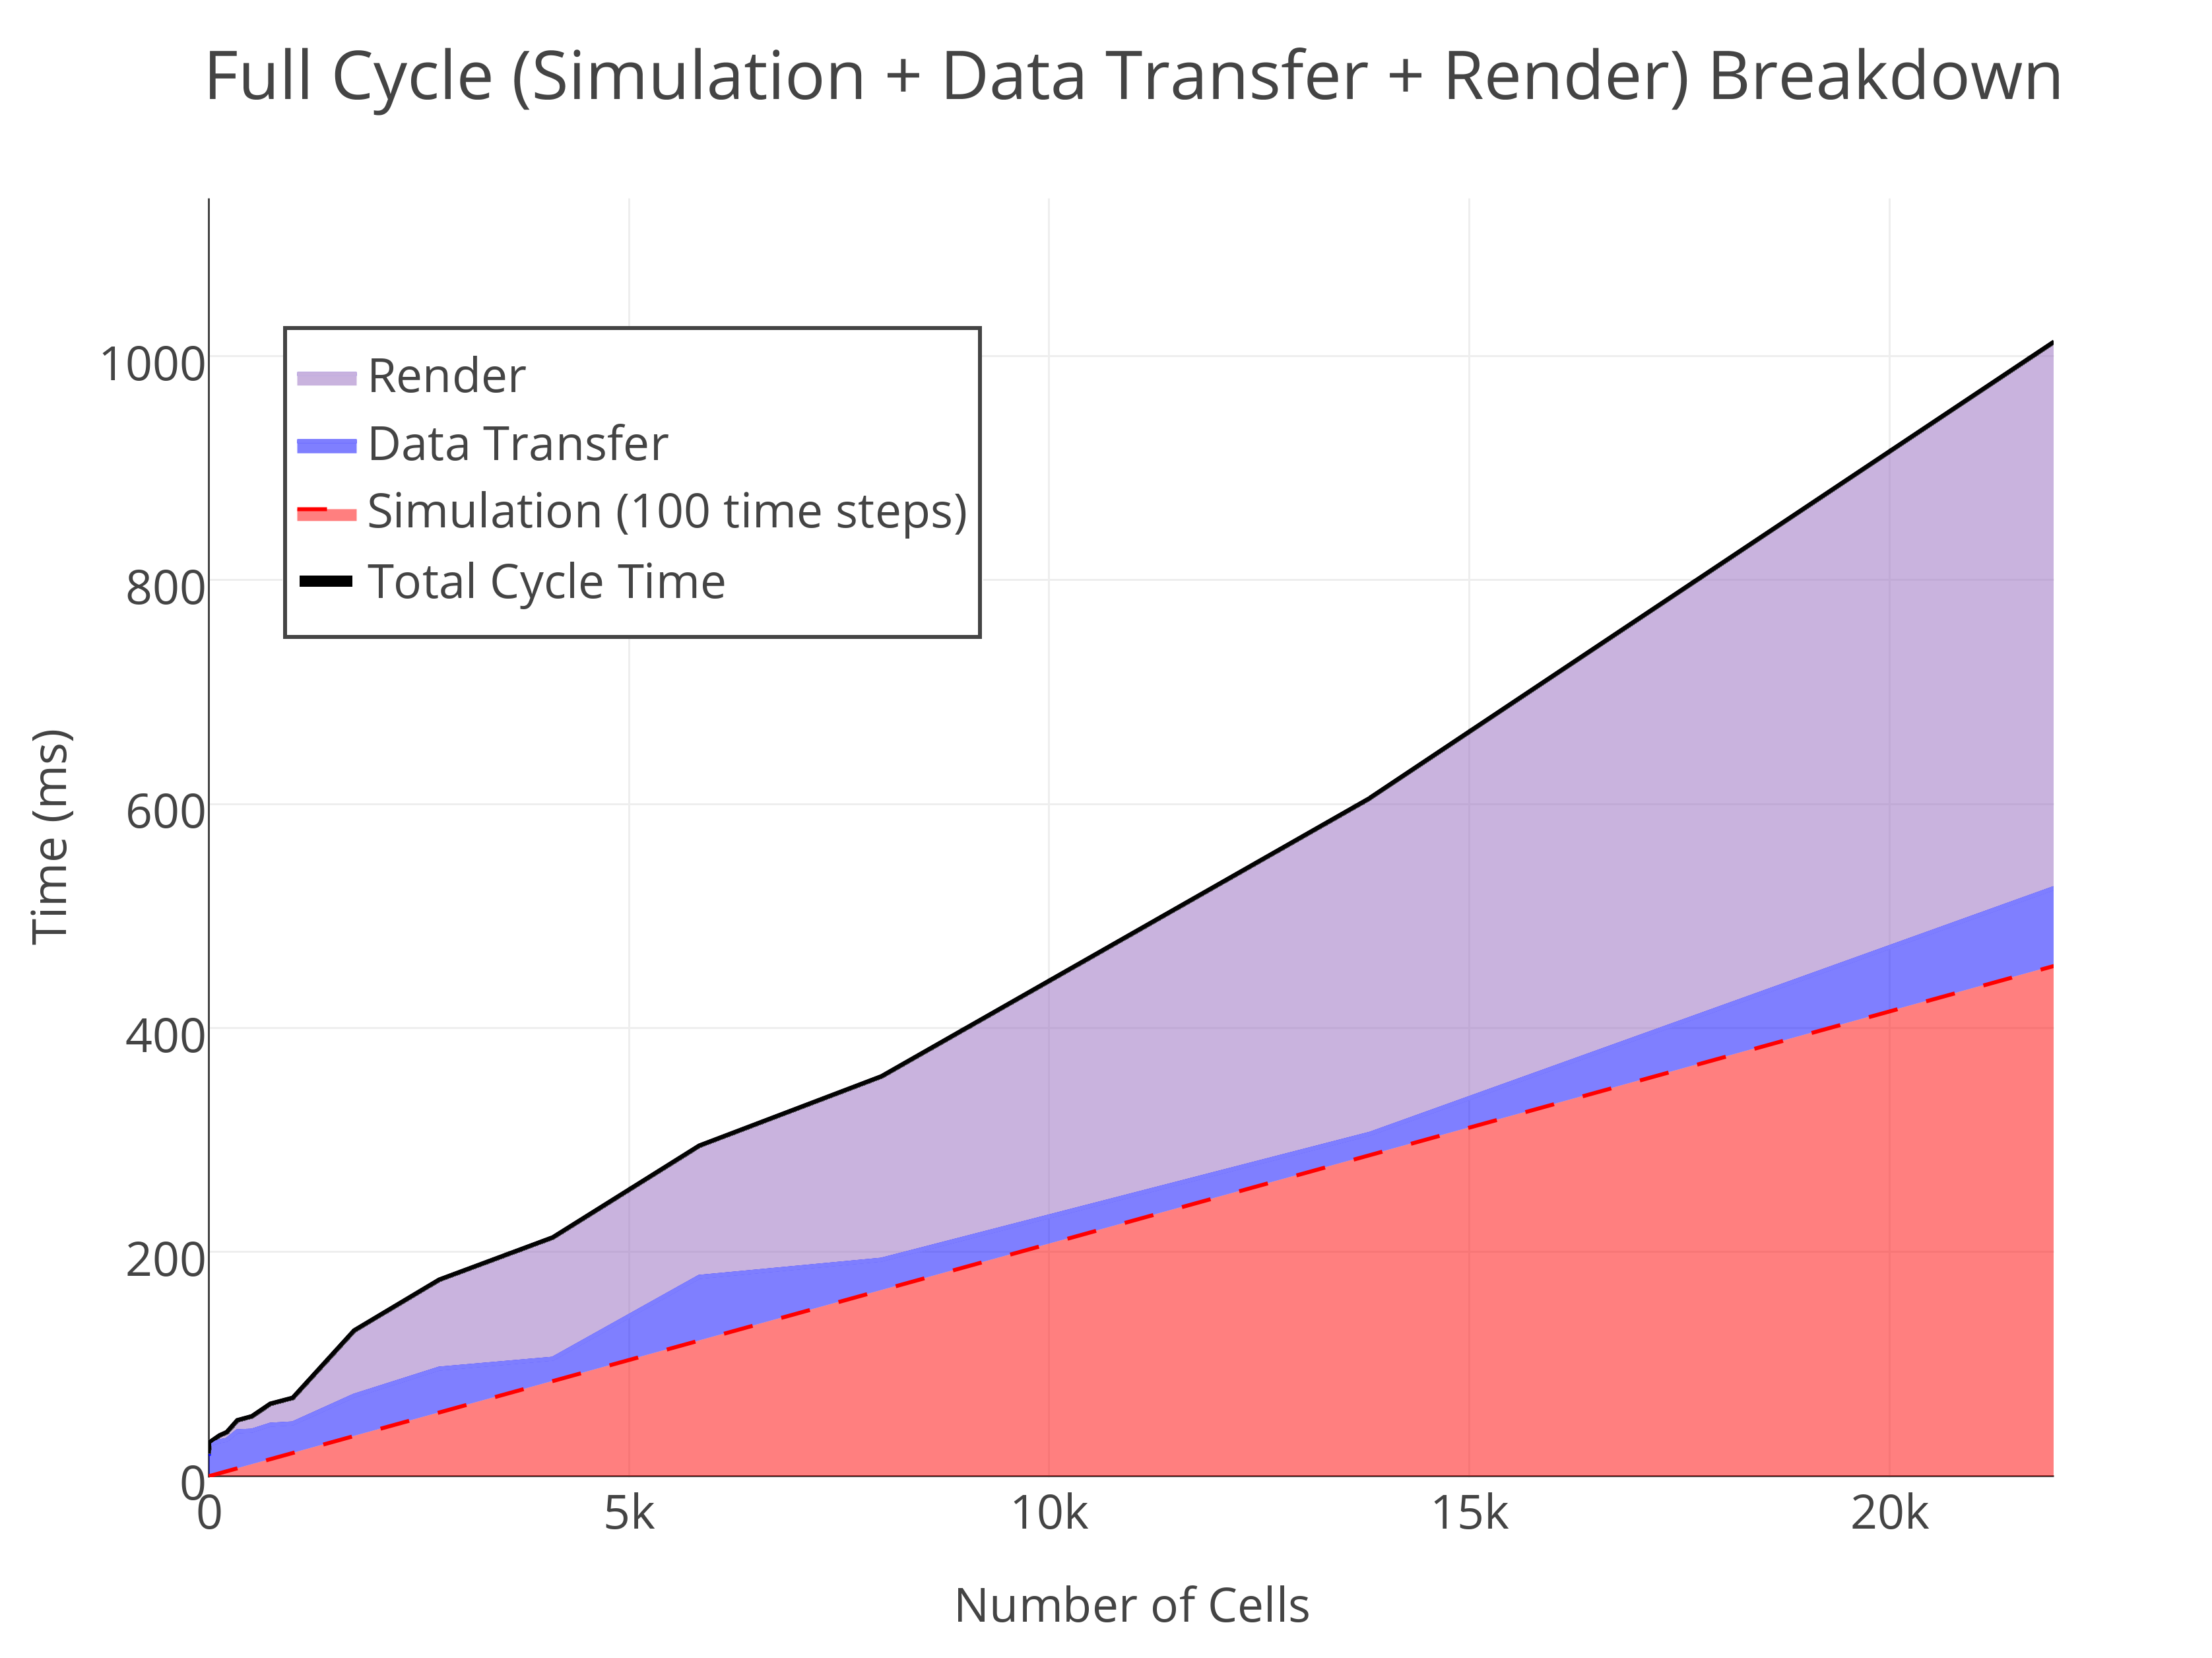
\includegraphics[width=\linewidth]{simcyclebreakdown.png}
  \caption{A breakdown of a full cycle of simulation (simulation + data transfer + rendering) shows where time was spent.  Time spent in 100 cycles of simulation (salmon), data transfer (blue), and rendering in threejs (purple) are shown in milliseconds.  Time to complete simulation was not measured directly, it was determined from analysis of Figure \ref{fig:simdatatransmetrics}.}
  \label{fig:simcyclebreakdown}
\end{figure}

Figure \ref{fig:simcyclebreakdown} shows the breakdown of a complete cycle in terms of time spent in simulation, data transfer, and rendering.  Data transfer takes about 30ms; this could be cut down by updating mesh positions and orientations on the GPU and bypassing data transfer completely.  Rendering speed could be improved greatly by removing invisible internal geometry and merging multiple geometries into a single threejs mesh.  I'm actually computing each interaction between cells twice - once when I process one cell, and again when I process its neighbor.  Since the forces and torques between neighboring cells are symmetric, no new information is gleaned from these extra calculations.  Removing this redundancy will decrease simulation processing time by some factor less than 0.5 depending on the connectivity of the assembly.  These optimizations will come after I'm through the debugging phase of this project.





